\def\year{2018}\relax
%File: formatting-instruction.tex
\documentclass[fleqn,10pt]{wlscirep} %DO NOT CHANGE THIS
% \usepackage{aaai18}  %Required
\usepackage{times}  %Required
\usepackage{helvet}  %Required
\usepackage{courier}  %Required
\usepackage{url}  %Required
\usepackage{graphicx}  %Required
% \frenchspacing  %Required
% \setlength{\pdfpagewidth}{8.5in}  %Required
% \setlength{\pdfpageheight}{11in}  %Required

\usepackage{xcolor}
%\usepackage{amsmath}
%\usepackage{verbatim}
%\usepackage{graphics}
\usepackage{subfig}
\usepackage{graphicx}
\usepackage{graphics}
\usepackage{multirow}
\usepackage{url}
%%decrease spacing 
\usepackage{times}
\usepackage{comment}
%
%\newtheorem{thm}{Theorem}
%\newtheorem{corr}{Corollary}
%\newtheorem{lemma}{Lemma}
%\newtheorem{pty}{Property}

\newcommand{\red}[1]{\textcolor{red}{#1}}
\newcommand{\blue}[1]{\textcolor{blue}{#1}}
\newcommand{\green}[1]{\textcolor{green}{#1}}
\newcommand{\sj}[1]{\green{#1}}
\newcommand{\ns}[1]{\red{#1}}


%PDF Info Is Required:
%\pdfinfo{
%	/Title (2018 Formatting Instructions for Authors Using LaTeX)
%	/Author (AAAI Press Staff)}
\setcounter{secnumdepth}{0}  
	% The file aaai.sty is the style file for AAAI Press 
	% proceedings, working notes, and technical reports.
	%
	
\title{Anatomy of support: Measuring properties of on-line supportive conversations}

\begin{abstract}
The boom in Internet connectivity has allowed people to express themselves using varied sets of networked media. This also involves people who express distress to seek help and comfort through the medium of  on-line forums and blogs. In this paper we try to dissect the dynamics through which distress calls are met in terms of conversational interactions and how they differ from a general non-supportive ones. We do so by first formalizing a graph based abstraction of nested conversations, considering the topical nature of replies to a message. We then relate different metrics that differentiate these conversations to a popular theory of community support. We specifically concentrate on conversations pertaining to expression of suicidal thoughts.  We experimentally show that supportive conversations are measurably different from generic ones using several topological measures and we discuss that these measures map well on the offline features of a supportive community. We show that supportive conversations are more urgent and involved and are carried on by an active topical discussion.  
\end{abstract}
\begin{document}
\flushbottom
\maketitle
\thispagestyle{empty}


\section{Introduction}
The world has become more connected over the past decades thanks to the networked nature of the technologies of the day. It is seldom possible to spend a whole day without single interaction on the Internet. The Internet gives platforms where we can not only connect with our social counterparts but also exchange ideas and express opinions. These new mediums have become so ubiquitous, that some research suggests that they might be affecting our broader psychological state \cite{d20122}. But on the positive side, studies have also proposed different ways in which this medium could be used for measuring and intervening in the matters of mental health\cite{DeChoudhury2016,DeChoudhury2014} 
One aspect of this is measuring signals and patterns in the data that are predictors of certain distresses. A good example\cite{DeChoudhury2014,DeChoudhury2016} looked at statistical relations of mental health and depression community with suicidal ideation. In their work, the authors explore linguistic and social characteristics that evaluate user's propensity to suicidal ideation. 
Another crucial and related work was carried out by \cite{gkotsis2017characterisation}, where they characterized mental health related posts on sub-reddit, and developed models to accurately predict type of condition based of informed language models.

In most cases, the work aimed at measuring signals of distress and not support, which is the complimentary part of the process and which make these on-line communities work. The only reason for expression of distress was because the users expect support from the community. In this work we measure the phenomenon of social support in online communities that deal with suicidal thoughts and suicidal expressions. We do this by a data driven study of Suicide Watch sub-reddit and baseline it using a large random collection of reddit threads from the Front page of the Reddit website. We in the process of measuring, try to ope rationalize a well establish theory on off-line support from literature \cite{minkler2005improving} using network topology and content features and show that the measures developed off-line hold true for this particular supportive community

%% SV: to add: condense the pubchline and the main methods and contributions. 5 main steps - network structure would be the typical network analysis which actually doesn't show anything in these datasets, but with the subsequent methods proposed here, significant differences are shown, and they provide a means to systematically analyze these types of communities
\section{Results}

We concentrate in a comparative study between Suicide Watch and the baseline, becasue this particular community has been
Particularly Suicide watch community consists of over 78k subscribers and reader, however is supported by mere 12 Moderators according to last count. These moderators are volunteers and do have a training, albeit through experience. All the moderators have been in that role for at least 3 years and the oldest goes as far as December 2008. 

As such it is valuable to understand how is a community like r/SuicideWatch thriving and in what aspects is this community similar or dis-similar from other casual subreddits. 

\subsection{Thread Engagement}
One thing to measure conversation was by difference or similarities in engagement with a thread in Subreddits. We look at two prime metrics, 1) Distribution of unique participants in a particular thread  2) Maximum Depth of a branch in the Reply graph of the thread . 
Figure \ref{fig:depthDist} shows the distribution of maximum depths across all Reply graphs for SW and AS subreddits. The SW theads depths have a median depth of 5 and mean of 7.5 compared to a median depth of 1 and mean of 1.7 for AS subreddits. This shows that on an average the longest branch of reply graphs for SW subreddits are much longer than the baseline subreddit. This is despite the fact that AskScience has a two order of magnitude advantage in terms of subscribed users (14,999,331) over Suicide watch(78,000). 

\begin{figure}[!ht]
	\centering
	% \hspace*{-5mm}
	\subfloat[]{
		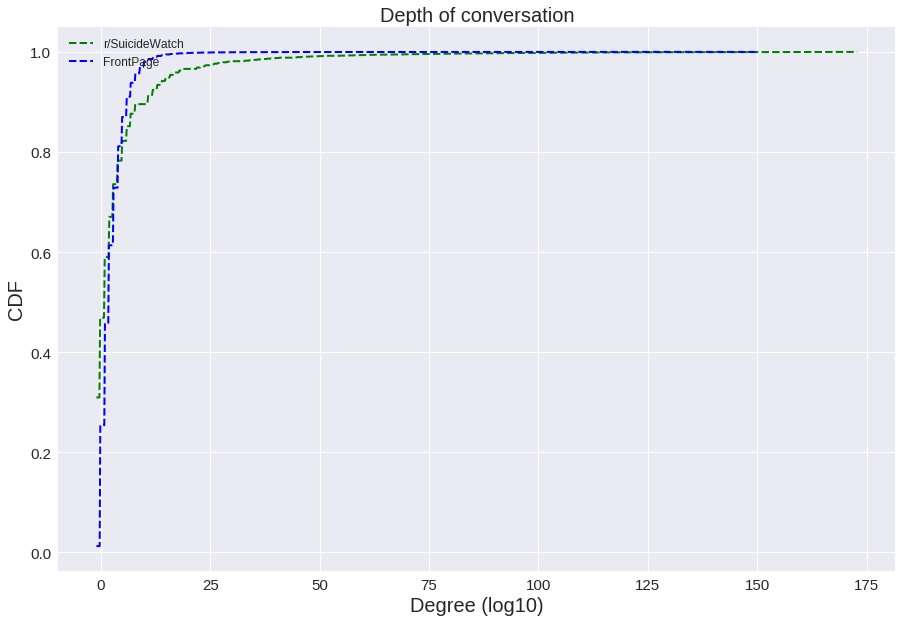
\includegraphics[width=0.45\textwidth, height = 5cm ]{Figures/DepthConversations.png}
		\label{fig:depthDist}
	}
	\subfloat[]{
		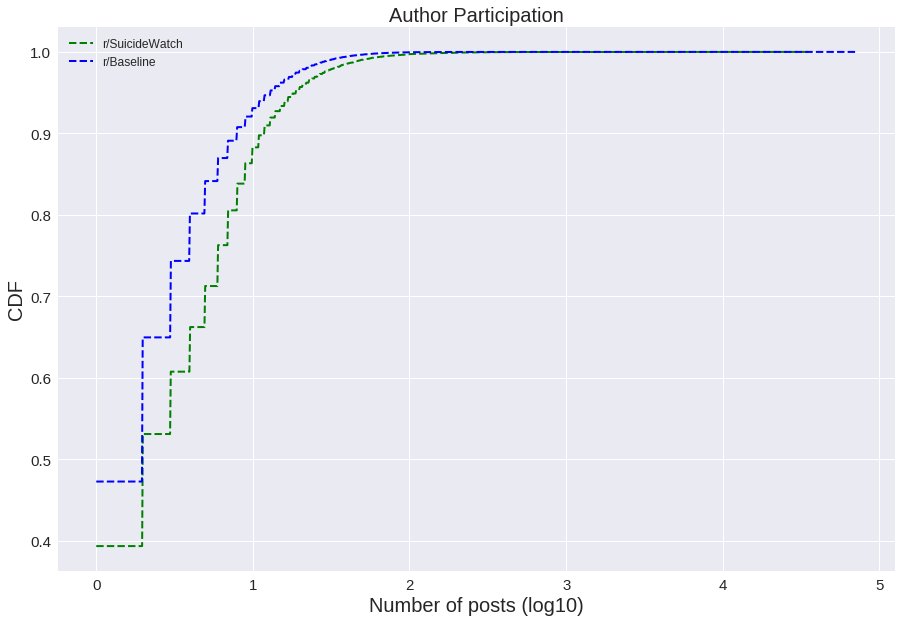
\includegraphics[width=0.45\linewidth, height = 5cm ]{Figures/AuthorParticipation.png}
		\label{fig:uniqAuthors}
	}
\caption{\textsl{ Fig \ref{fig:depthDist} shows the distribution of maximum depths of Reply Graphs for Subreddit r/SuicideWatch and the baseline Frontpage conversations. Fig \ref{fig:uniqAuthors} shows the distribution of unique authors per thread in the two datasets}}
\end{figure}



However if we  compare the number of unique users per thread, the two communities do not exibit much difference. SW subreddit has a median of 6 users per thread and a mean of 6.7 users and AS subreddit has a median of 5 users and mean of 13.3 users. So this shows than there is a somewhat uniform participation in terms of unique users responding to $RP$ on SW and a skewed but still at par participation on AS. 

\subsection{Network structure}
Because of the networked abstraction of threads as described in Sec \ref{Sec:Conversations}, we can now compare subreddits using network structural properties like degree distribution and structural holes in terms of conversations. 
Figures \ref{fig:repDegreeDist} and \ref{fig:userDegreeDist} show the comparison of degree distributions for both user and Reply graphs for two distinct sub-reddits. Despite having differences in terms of conversation depth, these two communities look similar in terms of classical degree distribution metrics. 

%% this illustration shows what a typical network analysis would be on a 'macro-level' which basically shows that there's no distintive difference between the two datasets, but if one looks at a micro-perspective (all analysis below), there's actually huge differences

\begin{figure}[!ht]
	\centering
	% \hspace*{-5mm}
	\subfloat[]{
		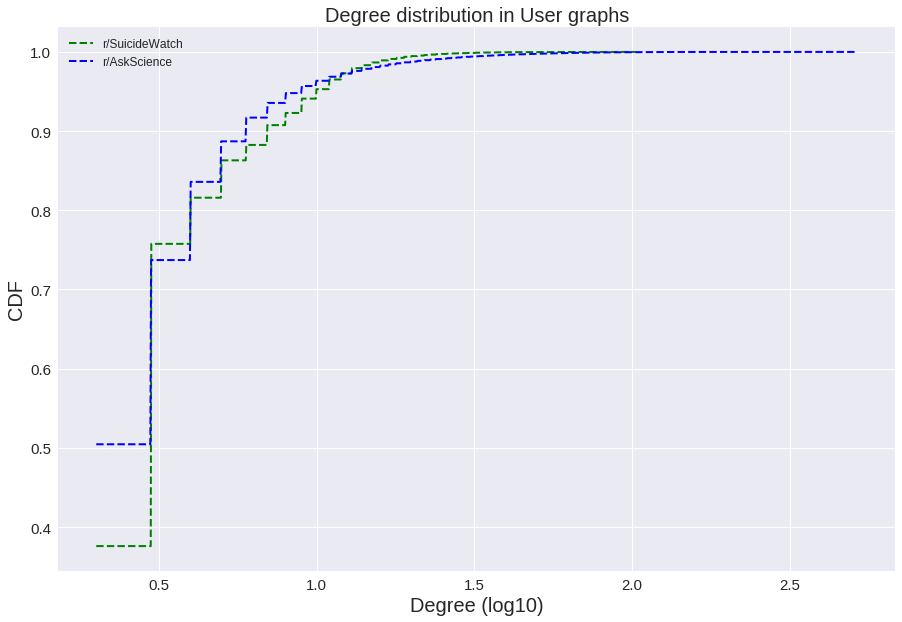
\includegraphics[width=0.45\textwidth, height = 5cm ]{Figures/degreeDistUgraph.png}
		\label{fig:rGraphSW}
	}
	\subfloat[]{
		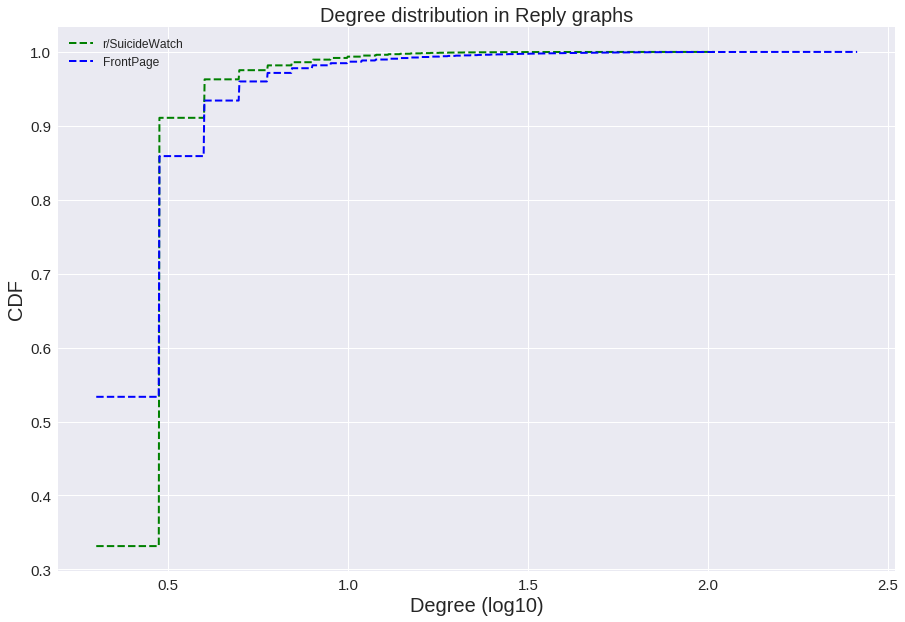
\includegraphics[width=0.45\linewidth, height = 5cm ]{Figures/degreeDistReplyGraph.png}
		\label{fig:uGraphSW}
	}
\caption{Fig \ref{fig:rGraphSW} shows Distribution of degrees for Reply Graphs,  r/SuicideWatch and FrontPage. Fig \ref{fig:uGraphSW} shows the degree distributions for the reply graphs}
\end{figure}

To compare the extent of similarity, we use the Mann-Whitey-U test. We calculate the test statistic across two sampled set of graphs taken from dataset of user and reply graphs for the baseline and SW subreddits. We then compare the cross dataset statistic with the statistic calculated between samples taken from the same dataset. This gives us an idea about similarity between two datasets. What we found that the distribution of degress for User and Reply graphs for SW and AS subreddits is up to 85\%. 

\subsection{Response Times}
Understanding the inter message times can act as a good proxy for the urgency in a conversation. To understand how Suicide watch subreddit users responds to a $OP$ compared to other sub-reddits like r/AskScience, we calculate differences between the posting times between consecutive messages in a reply graph. Figure \ref{fig:responseTimeDist} shows comparison using CDFs of inter-message response times for SW and AS subreddits. It can be seen that SW $OP$ are responded with the highest urgency amongst the 4, expecially compared to either the $OP$ or any other users or sub-reddits. 

\begin{figure}[!h]
	\centering
	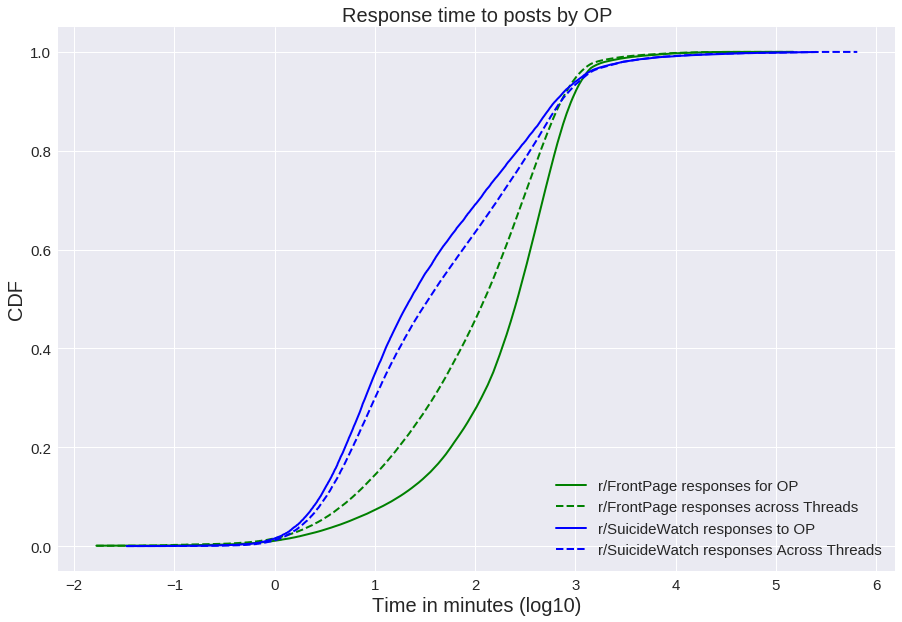
\includegraphics[width=0.5\columnwidth]{Figures/respTimeDist}
	\caption{\textsl{ CDF for the distribution of urgency if responses between two messages for OPs and across the forum. The comparison is between r/SuicideWatch and the Frontpage posts }}
	\label{fig:responseTimeDist}
\end{figure}

\subsection{Symmetric responses}
Despite signs of urgency and engagement, we ask the question: what percentage of conversations happening on these subreddits are symmetric in nature ? 
For this we first define a Symmetric user and a symmetric message. For a user $V_i$ in the user graph $G\{V,E,W\}$ as described in Section \ref{Sec:Conversations} , a symmetric user is a user who interacts with $V_o$ or the $OP$ and receives a response from the $OP$. We find the fraction $$U_{sym}=\frac{\textit{total number of symmetric users }}{\textit{Total users in a thread}}$$
Figure \ref{fig:symUsers} shows the CDF of $U_{sym}$ across the SW and AS sub-redditor.  The median value for $U_{sym}$ for SW is 20\% where as for AS is 0\%. This shows that SW subreddit engages is a lot more symmetric conversation that the baseline moderated subreddit like AS.



\begin{figure}[!h]
	\centering
	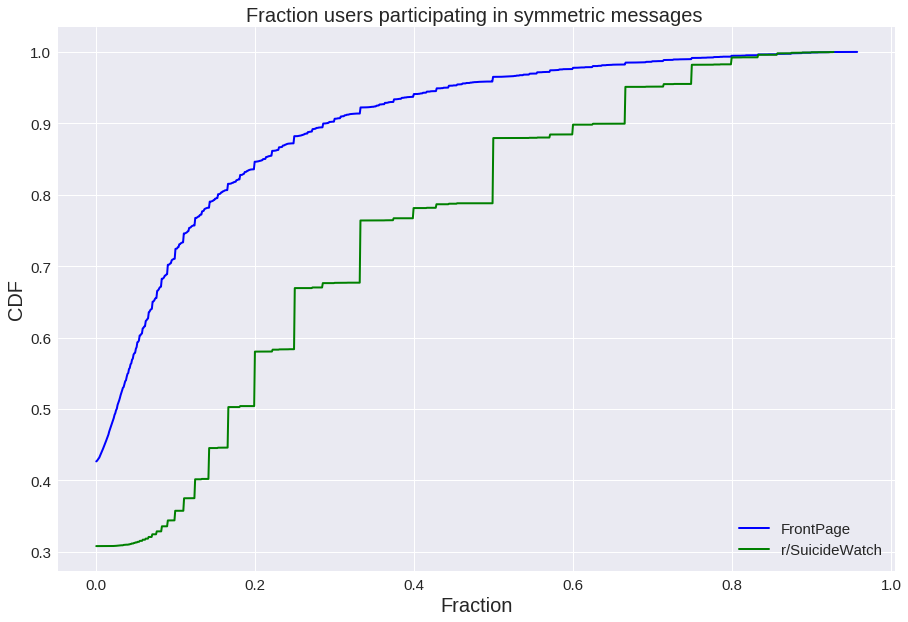
\includegraphics[width=0.5\columnwidth]{Figures/SymUsers.png}
	\caption{\textsl{ Figure shows Distribution of fraction of users in a thread participating in symmetric messaging for  r/SuicideWatch and FrontPage. }}
	\label{fig:symUsers}
\end{figure}


If we define a set of users who engage in symmetric activity with the $OP$ , it would be worth while to investigate how much of the total message activity on the thread is carried out by these set of symmetric users . To calculate this we find the fraction of messages on each thread written as part of this symmetric conversation. Figure \ref{fig:symMessages} shows the trend. It can be see that SW threads contain a higher prevalence of symmetric message exchanges compared to the baseline AS subreddit 

\subsection{Centralities}
To understand how embedded is the $OP$ in a conversation thread, we compare the betweenness centralities of $OPs$ in the $SW$ dataset with the baseline $FP$ dataset. 
Betweenness centralit of a node $v$ is defined as 
\begin{equation}
	g(v) = \sum_{s \neq v \neq t}\frac{\sigma_{st}(v)}{\sigma_{st}}
\end{equation}
where $\sigma_{st}(v)$ is the total number of shortest paths from node $s$ to node $t$ and $\sigma_{st}$ is the number of those paths that pass through $v$.


\begin{figure}[!h]
	\centering
	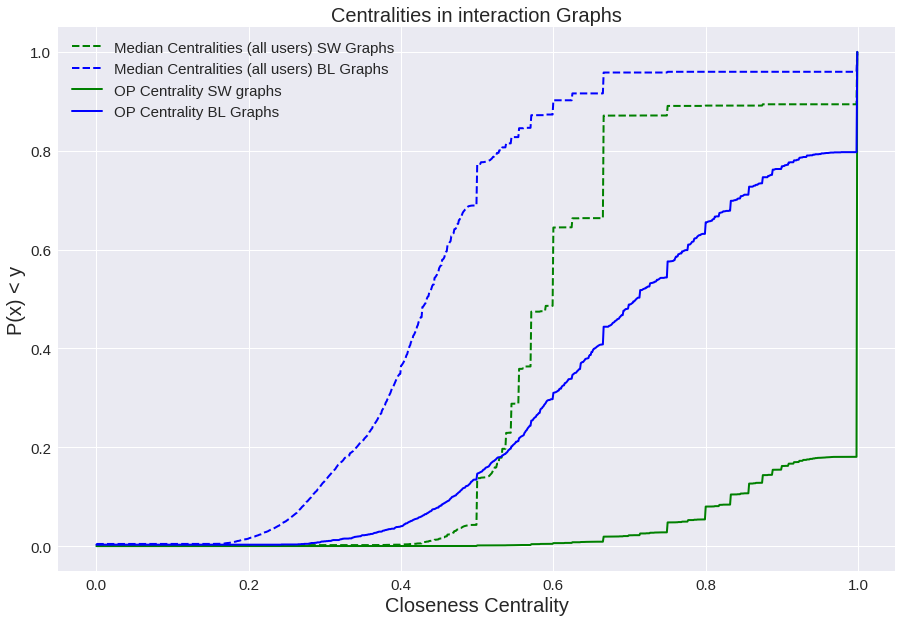
\includegraphics[width=0.5\columnwidth]{Figures/AllCentralities.png}
	\caption{\textsl{ CDF for Median Betweenness Centralities of all users in a conversation graph. The graph shows comparison between  to random threads from the Reddit $FP$ }}
	\label{fig:AllCentralities}
\end{figure}


Betweenness centrality is a good proxy of understanding how closely linked is a node with the rest of the network. When we calculate this metric for the user graphs we see that Suicide watch $OPs$ tend to have higher centralities compared to generic $FP$ threads. 


\subsection{Topical Alignment}

\begin{figure}[!h]
	\centering
	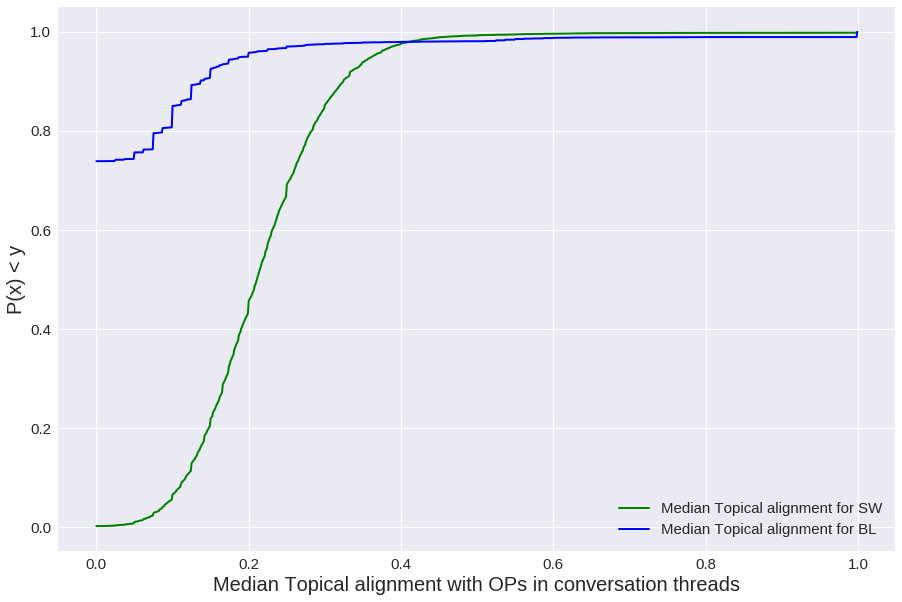
\includegraphics[width=0.5\columnwidth]{Figures/topicalAlignment.png}
	\caption{\textsl{ CDF for Median Betweenness Centralities of all users in a conversation graph. The graph shows comparison between  to random threads from the Reddit $FP$ }}
	\label{fig:TopicalAlignment}
\end{figure}


\subsection{Motif Analysis}

The figure \ref{fig:MotifOccurance} shows the results of the ratios of Baseline and Suicide watch across all 16 motifs. The motifs that deal with triadic closure like Motifs : 210 , 300 , 120D , 201 from Figure \ref{fig:motifs} are almost always over expressed in Suicide Watch. Check out Figures \ref{fig:210} , \ref{fig:300} , \ref{fig:120D}, and \ref{fig:201}. 


\begin{figure}[!ht]
	\centering
	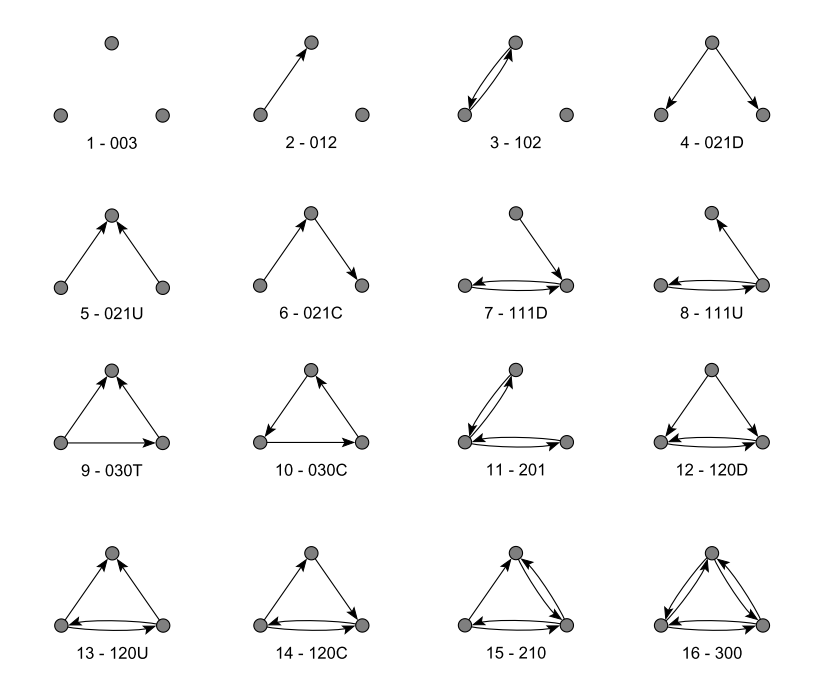
\includegraphics[width=0.7\textwidth]{Figures/TriadVariants}
	\caption{The 16 different types of motifs that are looked for in the user graph data.}
	\label{fig:motifs}
\end{figure}

\begin{figure*}[!t]
	\centering
	% \hspace*{-5mm}
	\subfloat[]{
		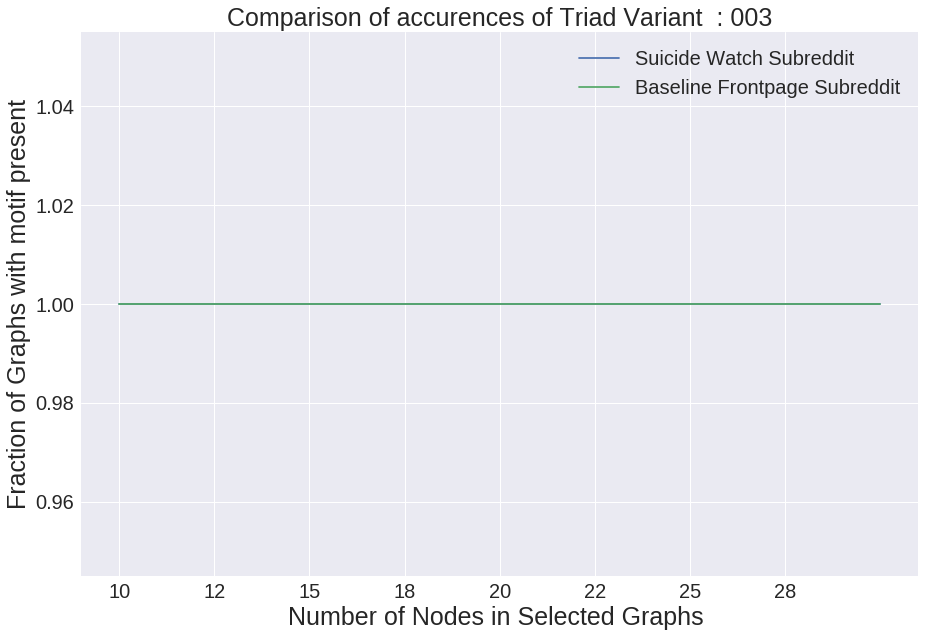
\includegraphics[width=0.22\textwidth, height = 3.5cm ]{Figures/003}
		\label{fig:003}
	}
	\subfloat[]{
		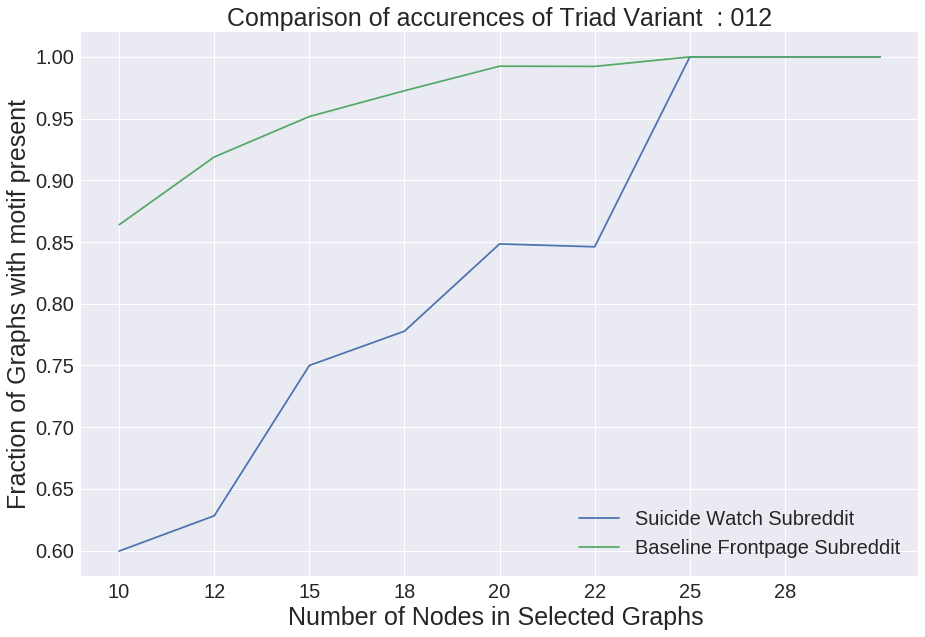
\includegraphics[width=0.22\linewidth, height = 3.5cm ]{Figures/012}
		\label{fig:012}
	}
	\subfloat[]{
		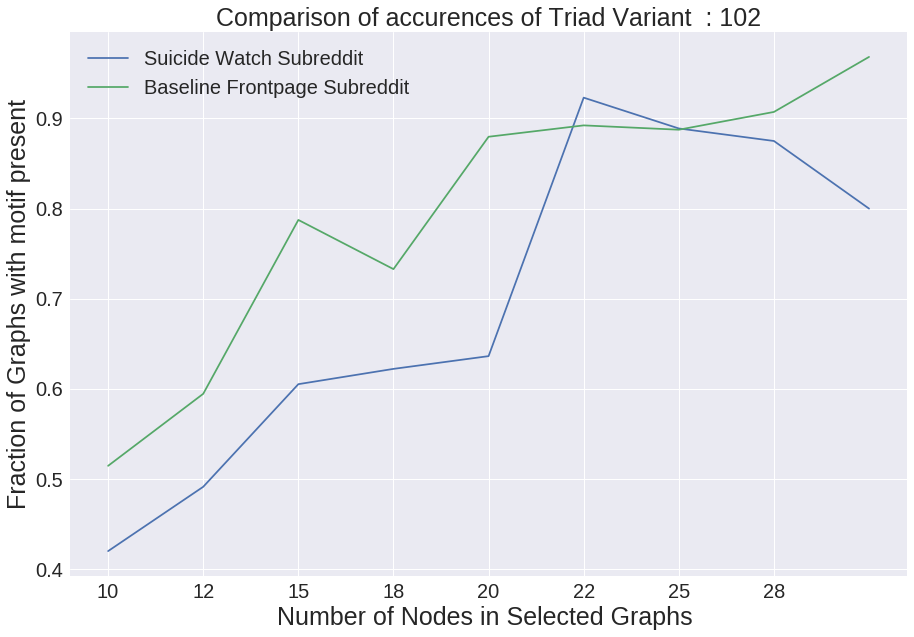
\includegraphics[width=0.22\linewidth, height = 3.5cm ]{Figures/102}
		\label{fig:102}
	}
	\subfloat[]{
		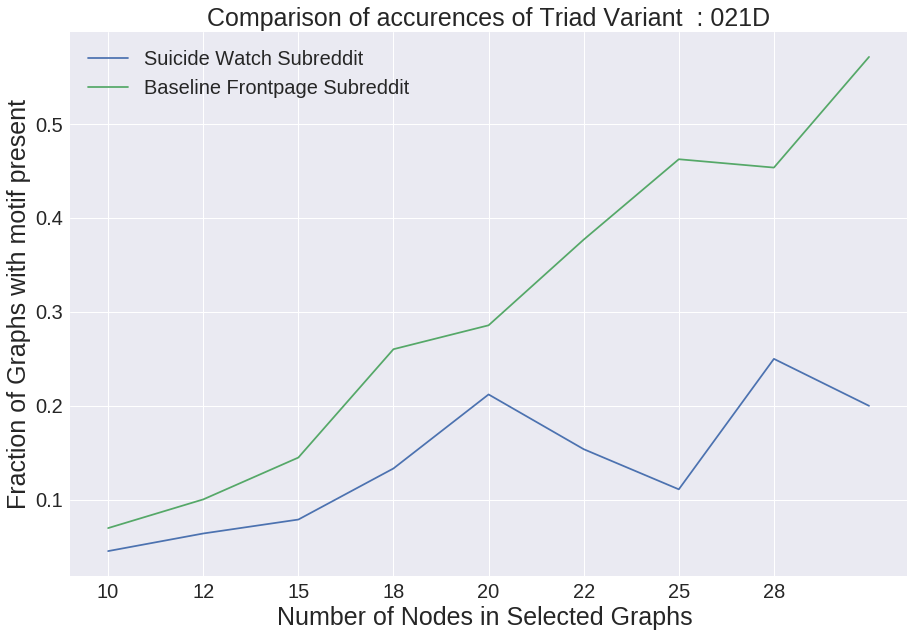
\includegraphics[width=0.22\linewidth, height = 3.5cm ]{Figures/021D}
		\label{fig:021D}
	}

	\subfloat[]{
	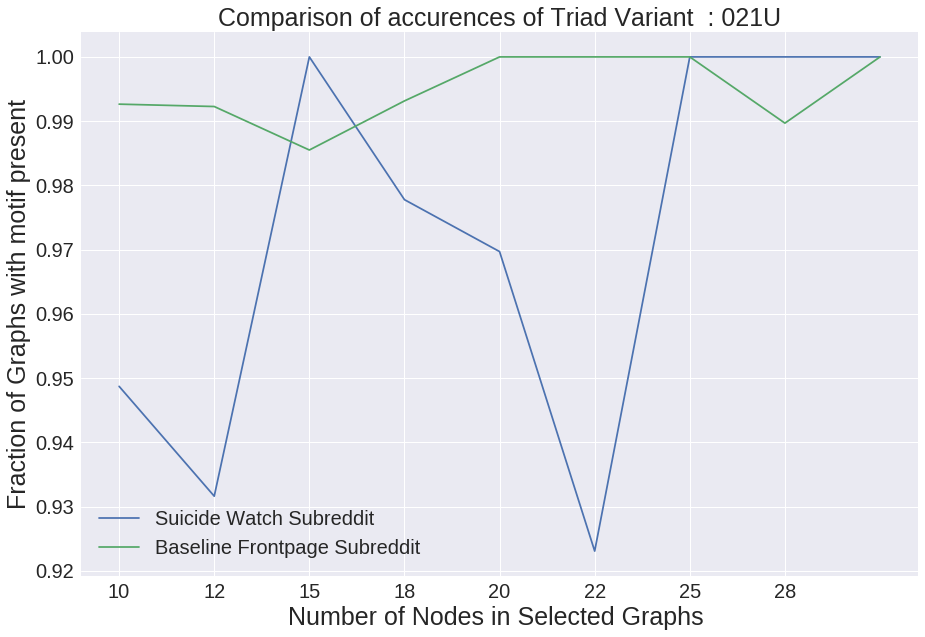
\includegraphics[width=0.22\linewidth, height = 3.5cm ]{Figures/021U}
	\label{fig:021U}
	}
	\subfloat[]{
	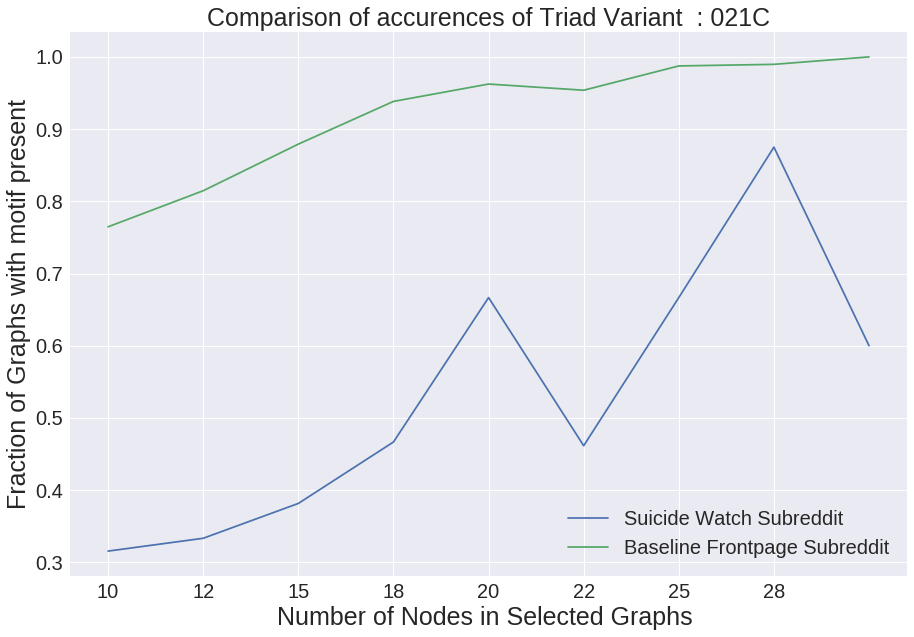
\includegraphics[width=0.22\linewidth, height = 3.5cm ]{Figures/021C}
	\label{fig:021C}
	}
	\subfloat[]{
	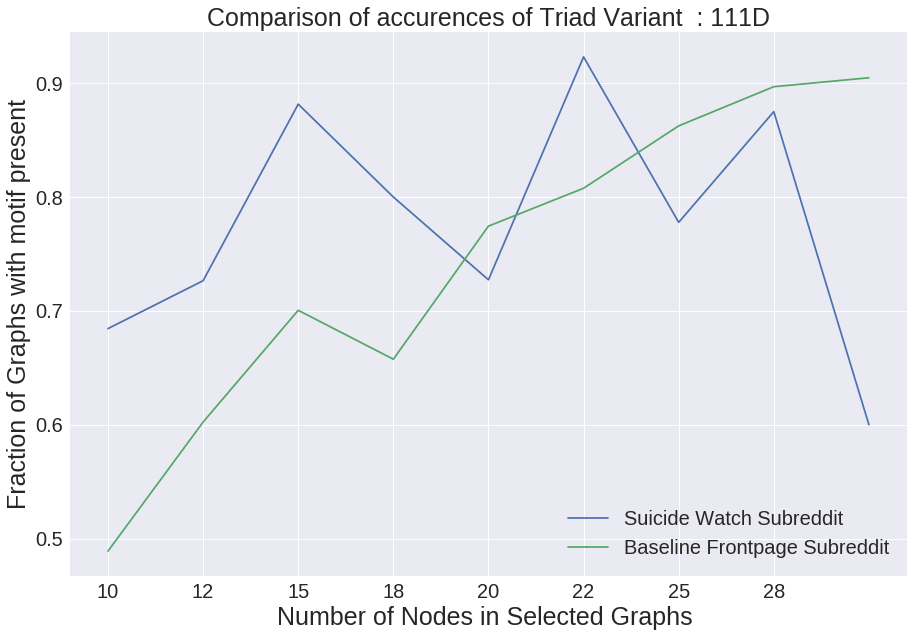
\includegraphics[width=0.22\linewidth, height = 3.5cm ]{Figures/111D}
	\label{fig:111D}
	}
	\subfloat[]{
	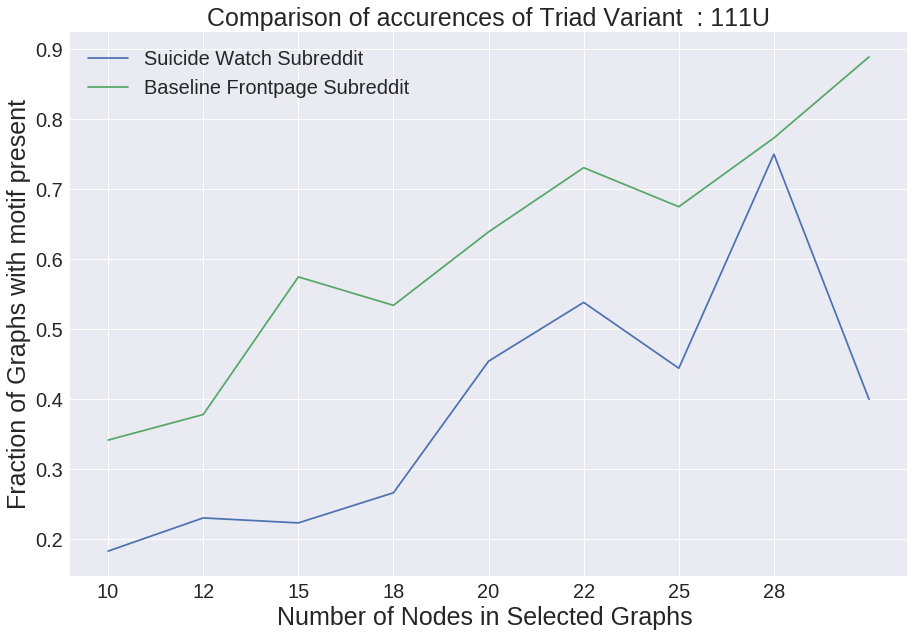
\includegraphics[width=0.22\linewidth, height = 3.5cm ]{Figures/111U}
	\label{fig:111U}
	}

	\subfloat[]{
	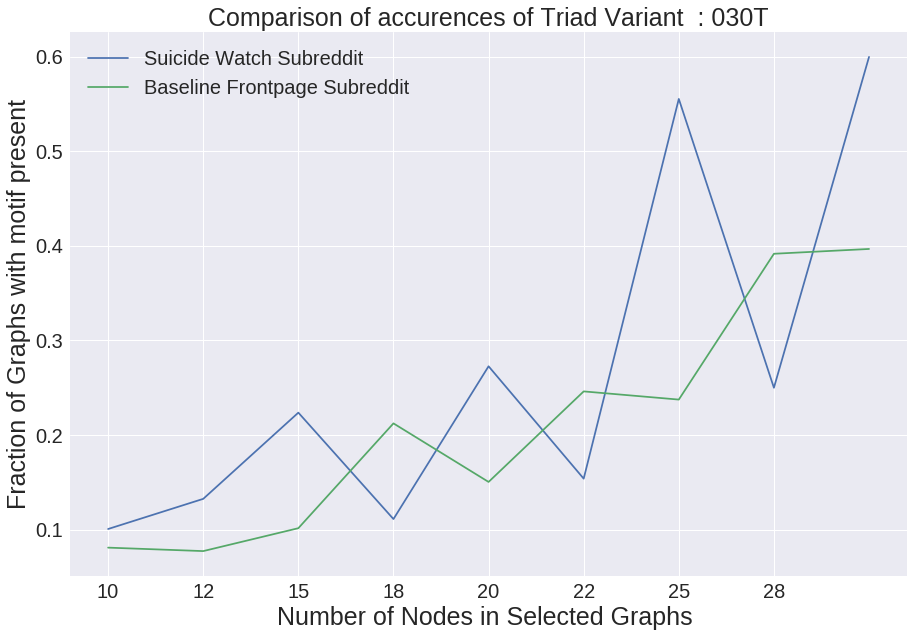
\includegraphics[width=0.22\linewidth, height = 3.5cm ]{Figures/030T}
	\label{fig:030T}
	}
	\subfloat[]{
	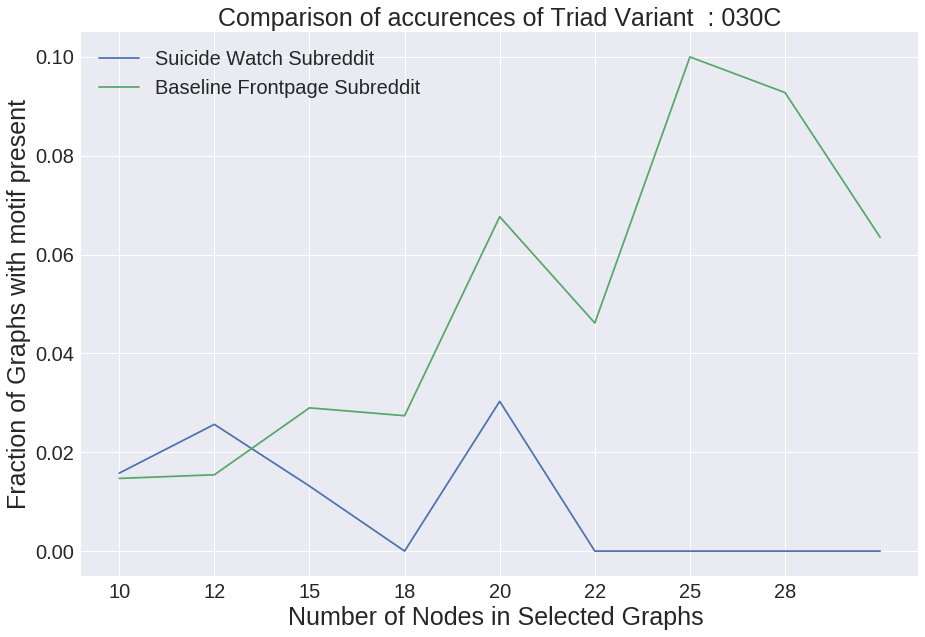
\includegraphics[width=0.22\linewidth, height = 3.5cm ]{Figures/030C}
	\label{fig:030C}
	}
	\subfloat[]{
	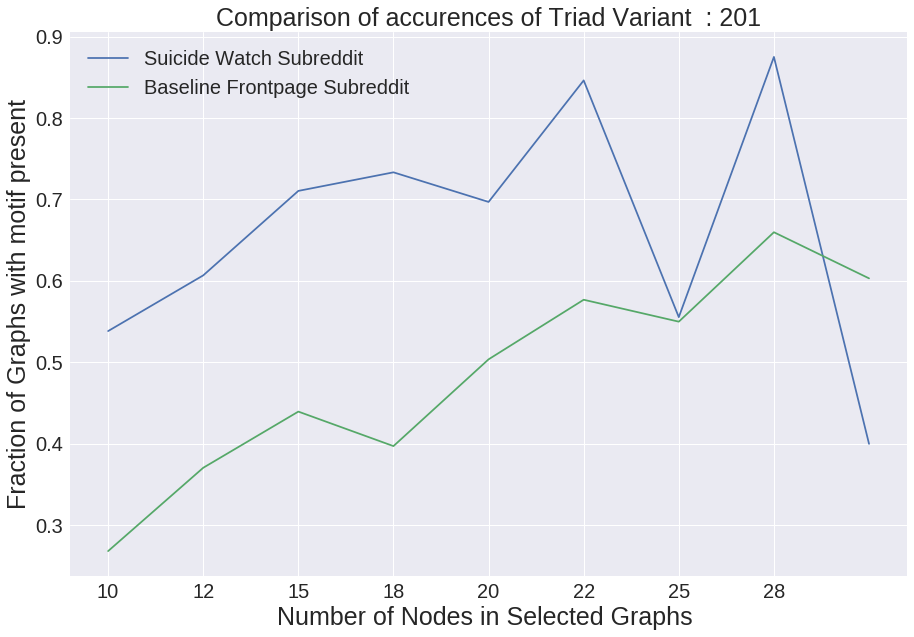
\includegraphics[width=0.22\linewidth, height = 3.5cm ]{Figures/201}
	\label{fig:201}
	}
	\subfloat[]{
	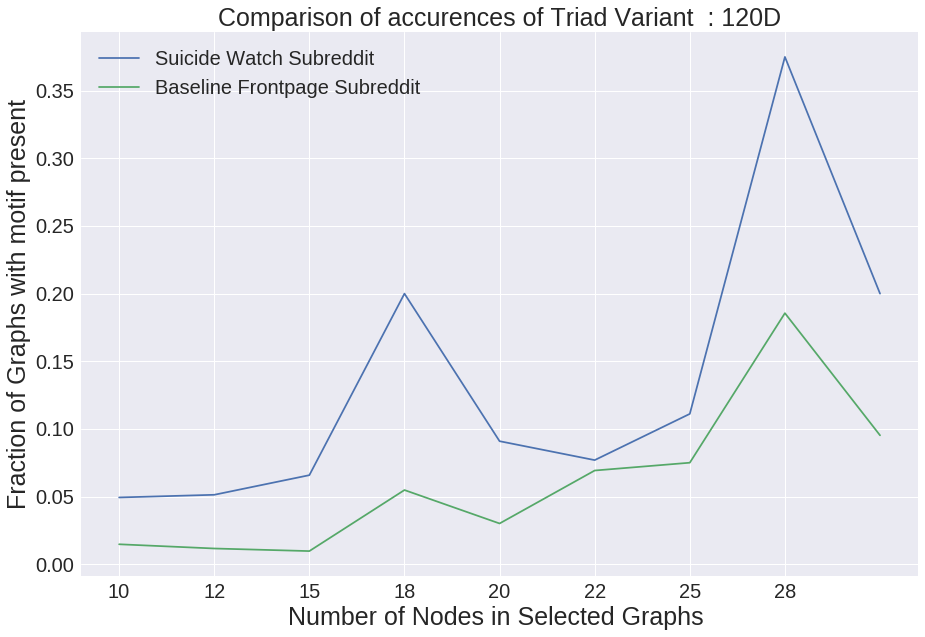
\includegraphics[width=0.22\linewidth, height = 3.5cm ]{Figures/120D}
	\label{fig:120D}
	}

	\subfloat[]{
	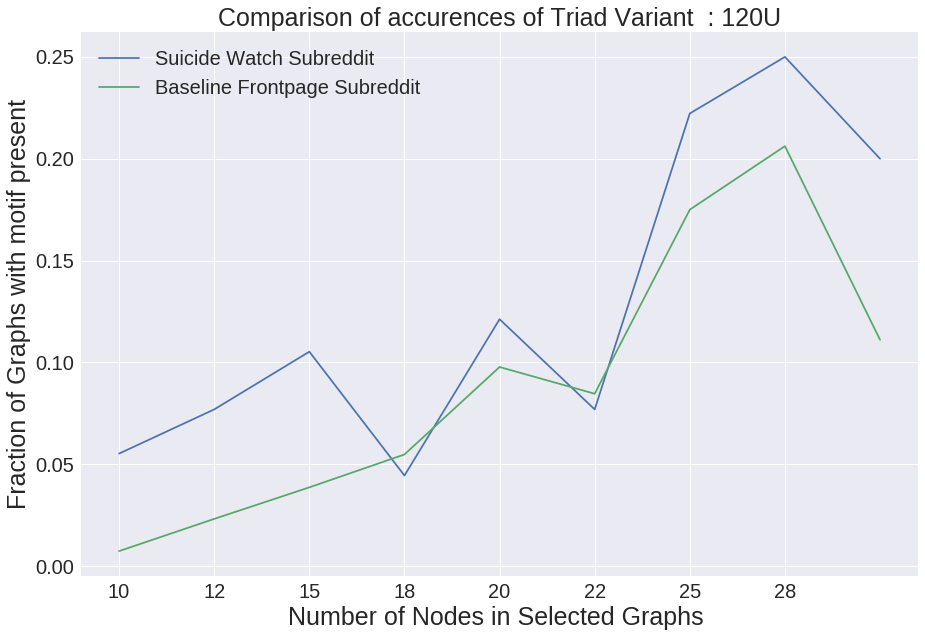
\includegraphics[width=0.22\linewidth, height = 3.5cm ]{Figures/120U}
	\label{fig:120U}
	}
	\subfloat[]{
	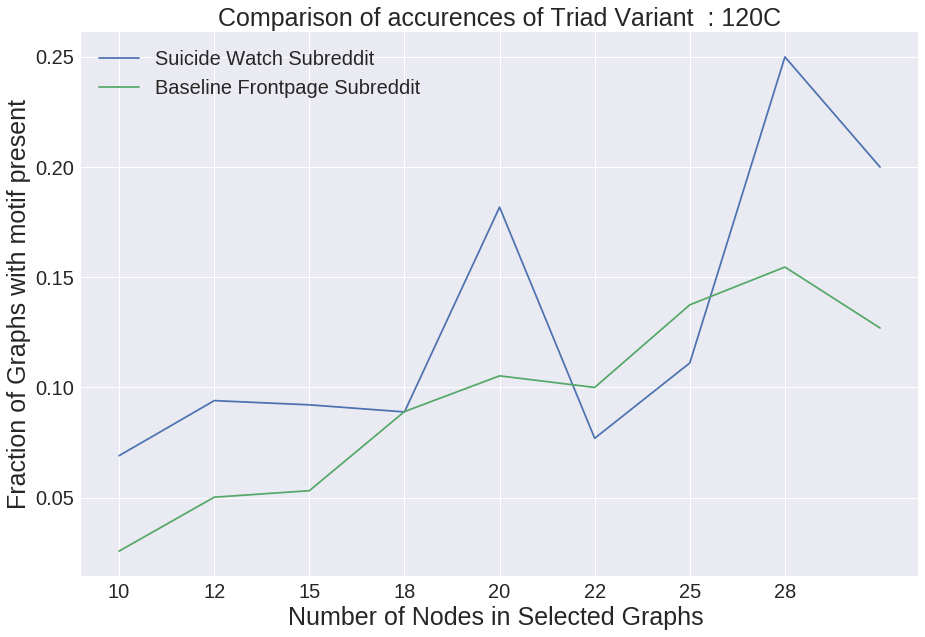
\includegraphics[width=0.22\linewidth, height = 3.5cm ]{Figures/120C}
	\label{fig:120C}
	}
	\subfloat[]{
	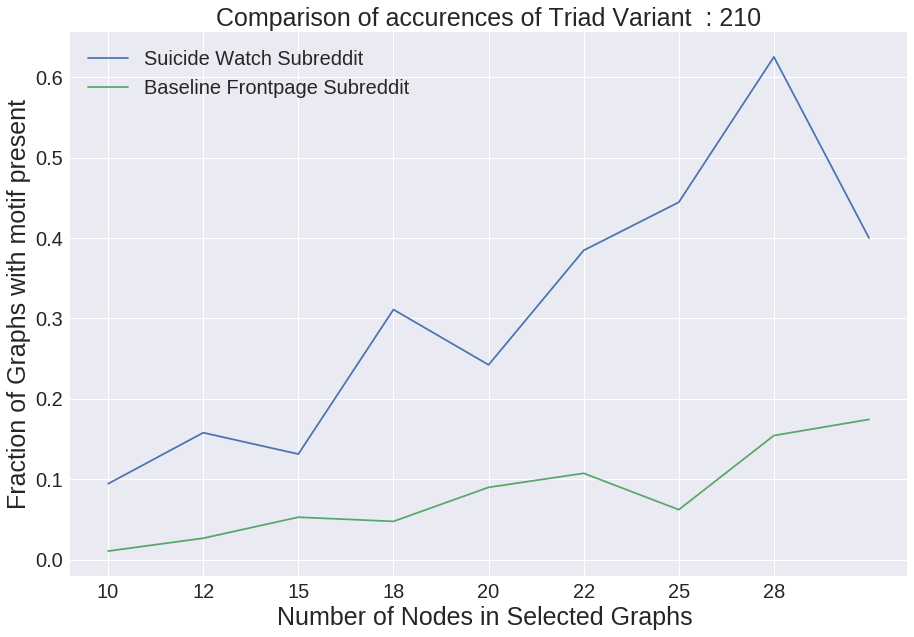
\includegraphics[width=0.22\linewidth, height = 3.5cm ]{Figures/210}
	\label{fig:210}
	}
	\subfloat[]{
	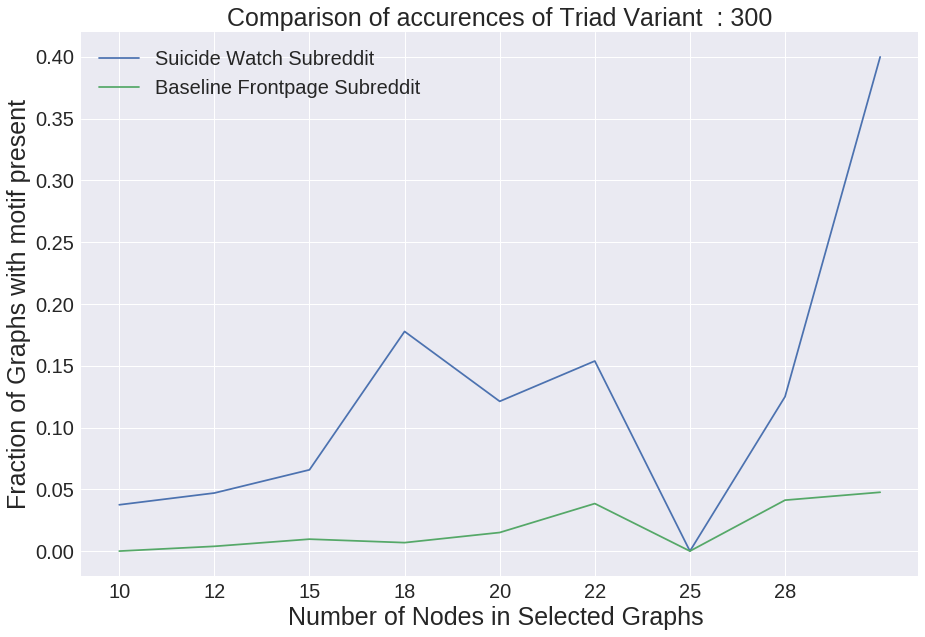
\includegraphics[width=0.22\linewidth, height = 3.5cm ]{Figures/300}
	\label{fig:300}
	}
	
	\label{fig:MotifOccurance}
	\vspace{-0.4cm}
	\caption{ The figure shows comparison of occurrence ratios of 16 motifs, one to one to figure \ref{fig:motifs}. Blue traces are for Suicide watch and Green traces are for Baseline Front pages}
	\vspace{-0.4cm}
\end{figure*}
\section{Discussion}
\section{Methods}
\subsection{Data}
We build on dataset that was used in \cite{gkotsis2017characterisation} where they analyze textual content for the root posts in a Subreddit called Suicide Watch\footnote{\url{https://www.reddit.com/r/SuicideWatch/}}. The dataset contains a dump of 53 thousand posts from the suicide watch sub-reddit. 
However the dataset did not contain the threaded conversations for each thread. Reddit is a platform where a user can create a post on a sub-reddit, to which several members of a given sub-reddit can interact with. The array of interactions may range from simple up or down votes or posting at different hierarchy of the thread. This creates a hierarchical threaded structure of posts where the conversations are organized as threads of posts. To understand the deeper nature of these posts,  we crawl Reddit to get the threaded conversations\footnote{The code to crawl reddit for threads can be found at \textit{https://github.com/sagarjoglekar/redditTools}} 

To baseline our work and compare theorized supportive nature of conversations with the broader community, we also crawl other reddit threads. To avoid any bias towards a particular type of subreddit, which have their own culture, we acquire roughly 50 thousand baseline posts which have been popular enough to land on the front page \footnote{The reddit front page algorithm is a combination of popularity and decay in popularity as a function of time. More can be found here \url{https://goo.gl/uVdHjn}}. We crawl the Frontpage posts for 2 weeks accumulating over 50 thousand reddit threads in the process. 

Figure\ref{fig:responseDist} shows the CDF for the number of responses a Root post gets on a thread across the whole dataset. 
\begin{figure}[!htb]
	\centering
	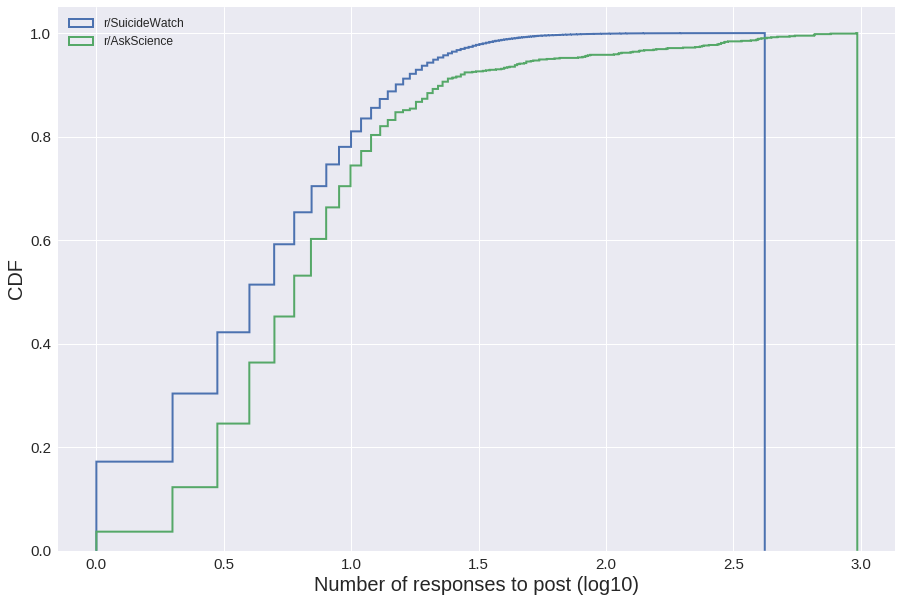
\includegraphics[width=0.5\columnwidth]{Figures/responseDistSW}
	\caption{\textsl{ Distribution of responses per thread on Subreddits r/SuicideWatch and r/AskScience }}
	\label{fig:responseDist}
\end{figure}

Figure \ref{fig:responseDist} shows the CDF for number of comments per thread across the r/SuicideWatch subreddit dataset and the crawled frontpage subreddit. 


\subsection{Abstraction: Networked conversations}

\begin{table}
	\resizebox{0.7\linewidth}{!}{
		\begin{tabular}{l|p{8cm}}
			\textbf{Terminology} & \textbf{stands for}\\
			$RP$   & Root post which begins a new thread on a subreddit \\
			$OP$  & Original poster who posts the Root post for a thread \\
			$BP$   & A Poster who has at-least one symmetric response from the $OP$ after his comment\\
			$AP$   & Asymmetric poster who responds to $OP$ but never gets a response back \\
			$SW$ & The suicide watch Subreddit \\
			$FP$  & Front page of Reddit. \\
			$TD$ & The Donald Subreddit \\
			$AS$ & AskScience subreddit \\
	\end{tabular}}
	\caption{Notations and Terms.}\label{notations}
\end{table}


\label{Sec:Conversations}
To understand the dynamics of supportive conversations, we first need to formalize the abstraction of networked conversations. In case of forum based platforms where users interact in a nested dialogue fashion, and original poster or $OP$ posts a start of a thread. This thread is then open for comments by all the community users. In case of Reddit, such a community is called a Subreddit, which is a moderated collection of users who subscribe to it. These users may post new threads onto the subreddit as far as the post follows the subreddit rules. Enforcement of these rules is the responsibility of the moderators. 

The user who starts a thread is called the Original Poster or $OP$ and the headlining post which the $OP$ begins with is called the Root Post or $RP$. We represent the data using two abstractions. One abstraction is called the \textbf{User Graphs} abstraction. In this method, we represent each thread as a directed graph $G\{V,E,W\}$ where $V$ is the set of all users participating in a particular thread and $E$ are the directed  edges which correspond to interactions between two users $V_i , V_j  \in V$. The weight of each directed edge $E_{ij}$ corresponds to the average Jaccard coefficient calculated on topics covered by posts done by $V_i$ to user $V_J$. 
Formally if $T_i$ is the content of the post posted by $V_i$ and $T_j$ is the content of the post posted by $V_j$ and if $F$ is a topic model trained on the corpus of all texts such that $F(T) \mapsto [t_0 , t_1 \ldots t_n ]$ where $t_k$ is the topic that is present in text $T$, then 
\begin{equation}
	W_{ij} = \frac{F(T_i) \cap F(T_j)}{F(T_i) \cup F(T_j)}
\end{equation}
Where $W_{ij}$ is the edge weight between node $V_i$ and node $V_j$.

The Second abstraction to work with in this paper is the \textbf{Reply Graph} abstraction. We formulate a reply graph $R\{P,E\}$ as a thread of multi-layered posts in a thread in response to the root post $RP$ in the sub-reddit. Each graph $R$ consists of posts $P_i , P_j , i,j \in N$ , where N+1 is the total number of responses in the thread and Edges $E_{ij}$such that and Edge $E_{ij}$ exists $iff$ post $P_i$ was in response to post $P_j$ in the hierarchy of responses. This abstraction works well in modelling the conversational nature of these forums.  For convienece of the reader, we present a couple of example pairs from SW and TheDonald subreddit in Figure \ref{Fig:GraphExamples}
\begin{figure*}[!ht]
	\centering
	% \hspace*{-5mm}
	\subfloat[]{
		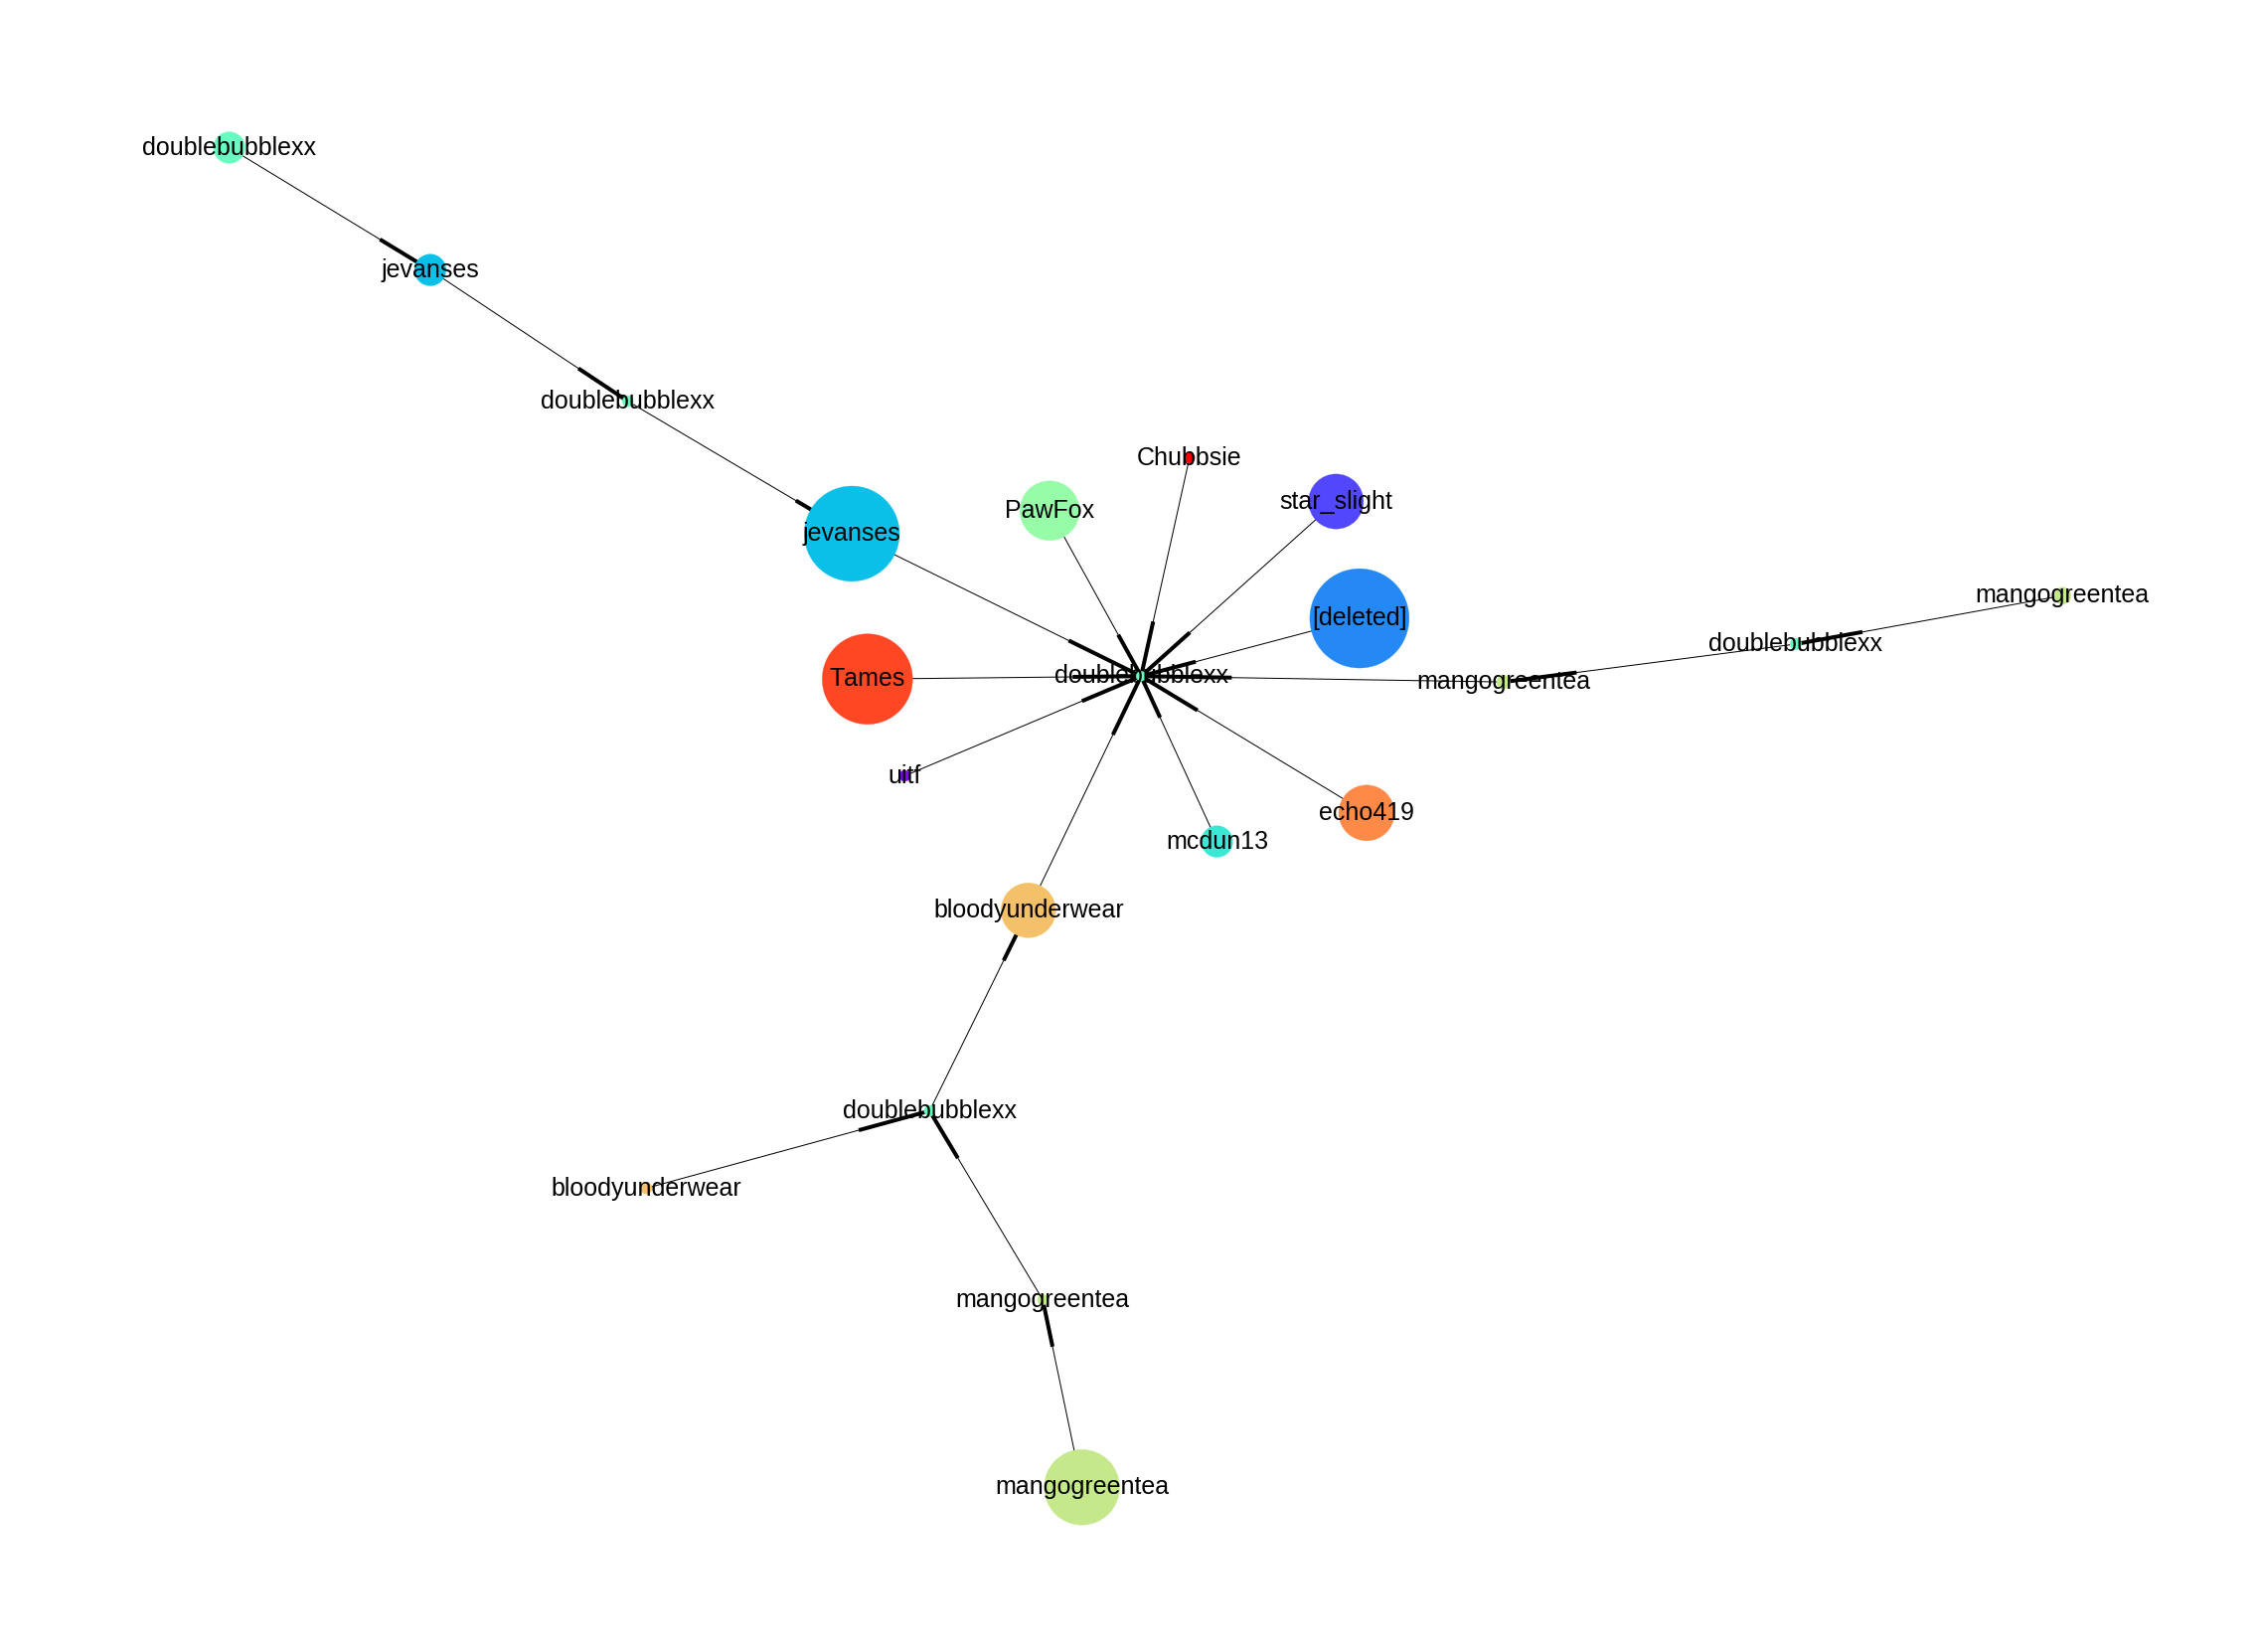
\includegraphics[width=0.45\textwidth, height = 5cm ]{Figures/ReplyGraphSW}
		\label{fig:rGraphSW}
	}
	\subfloat[]{
		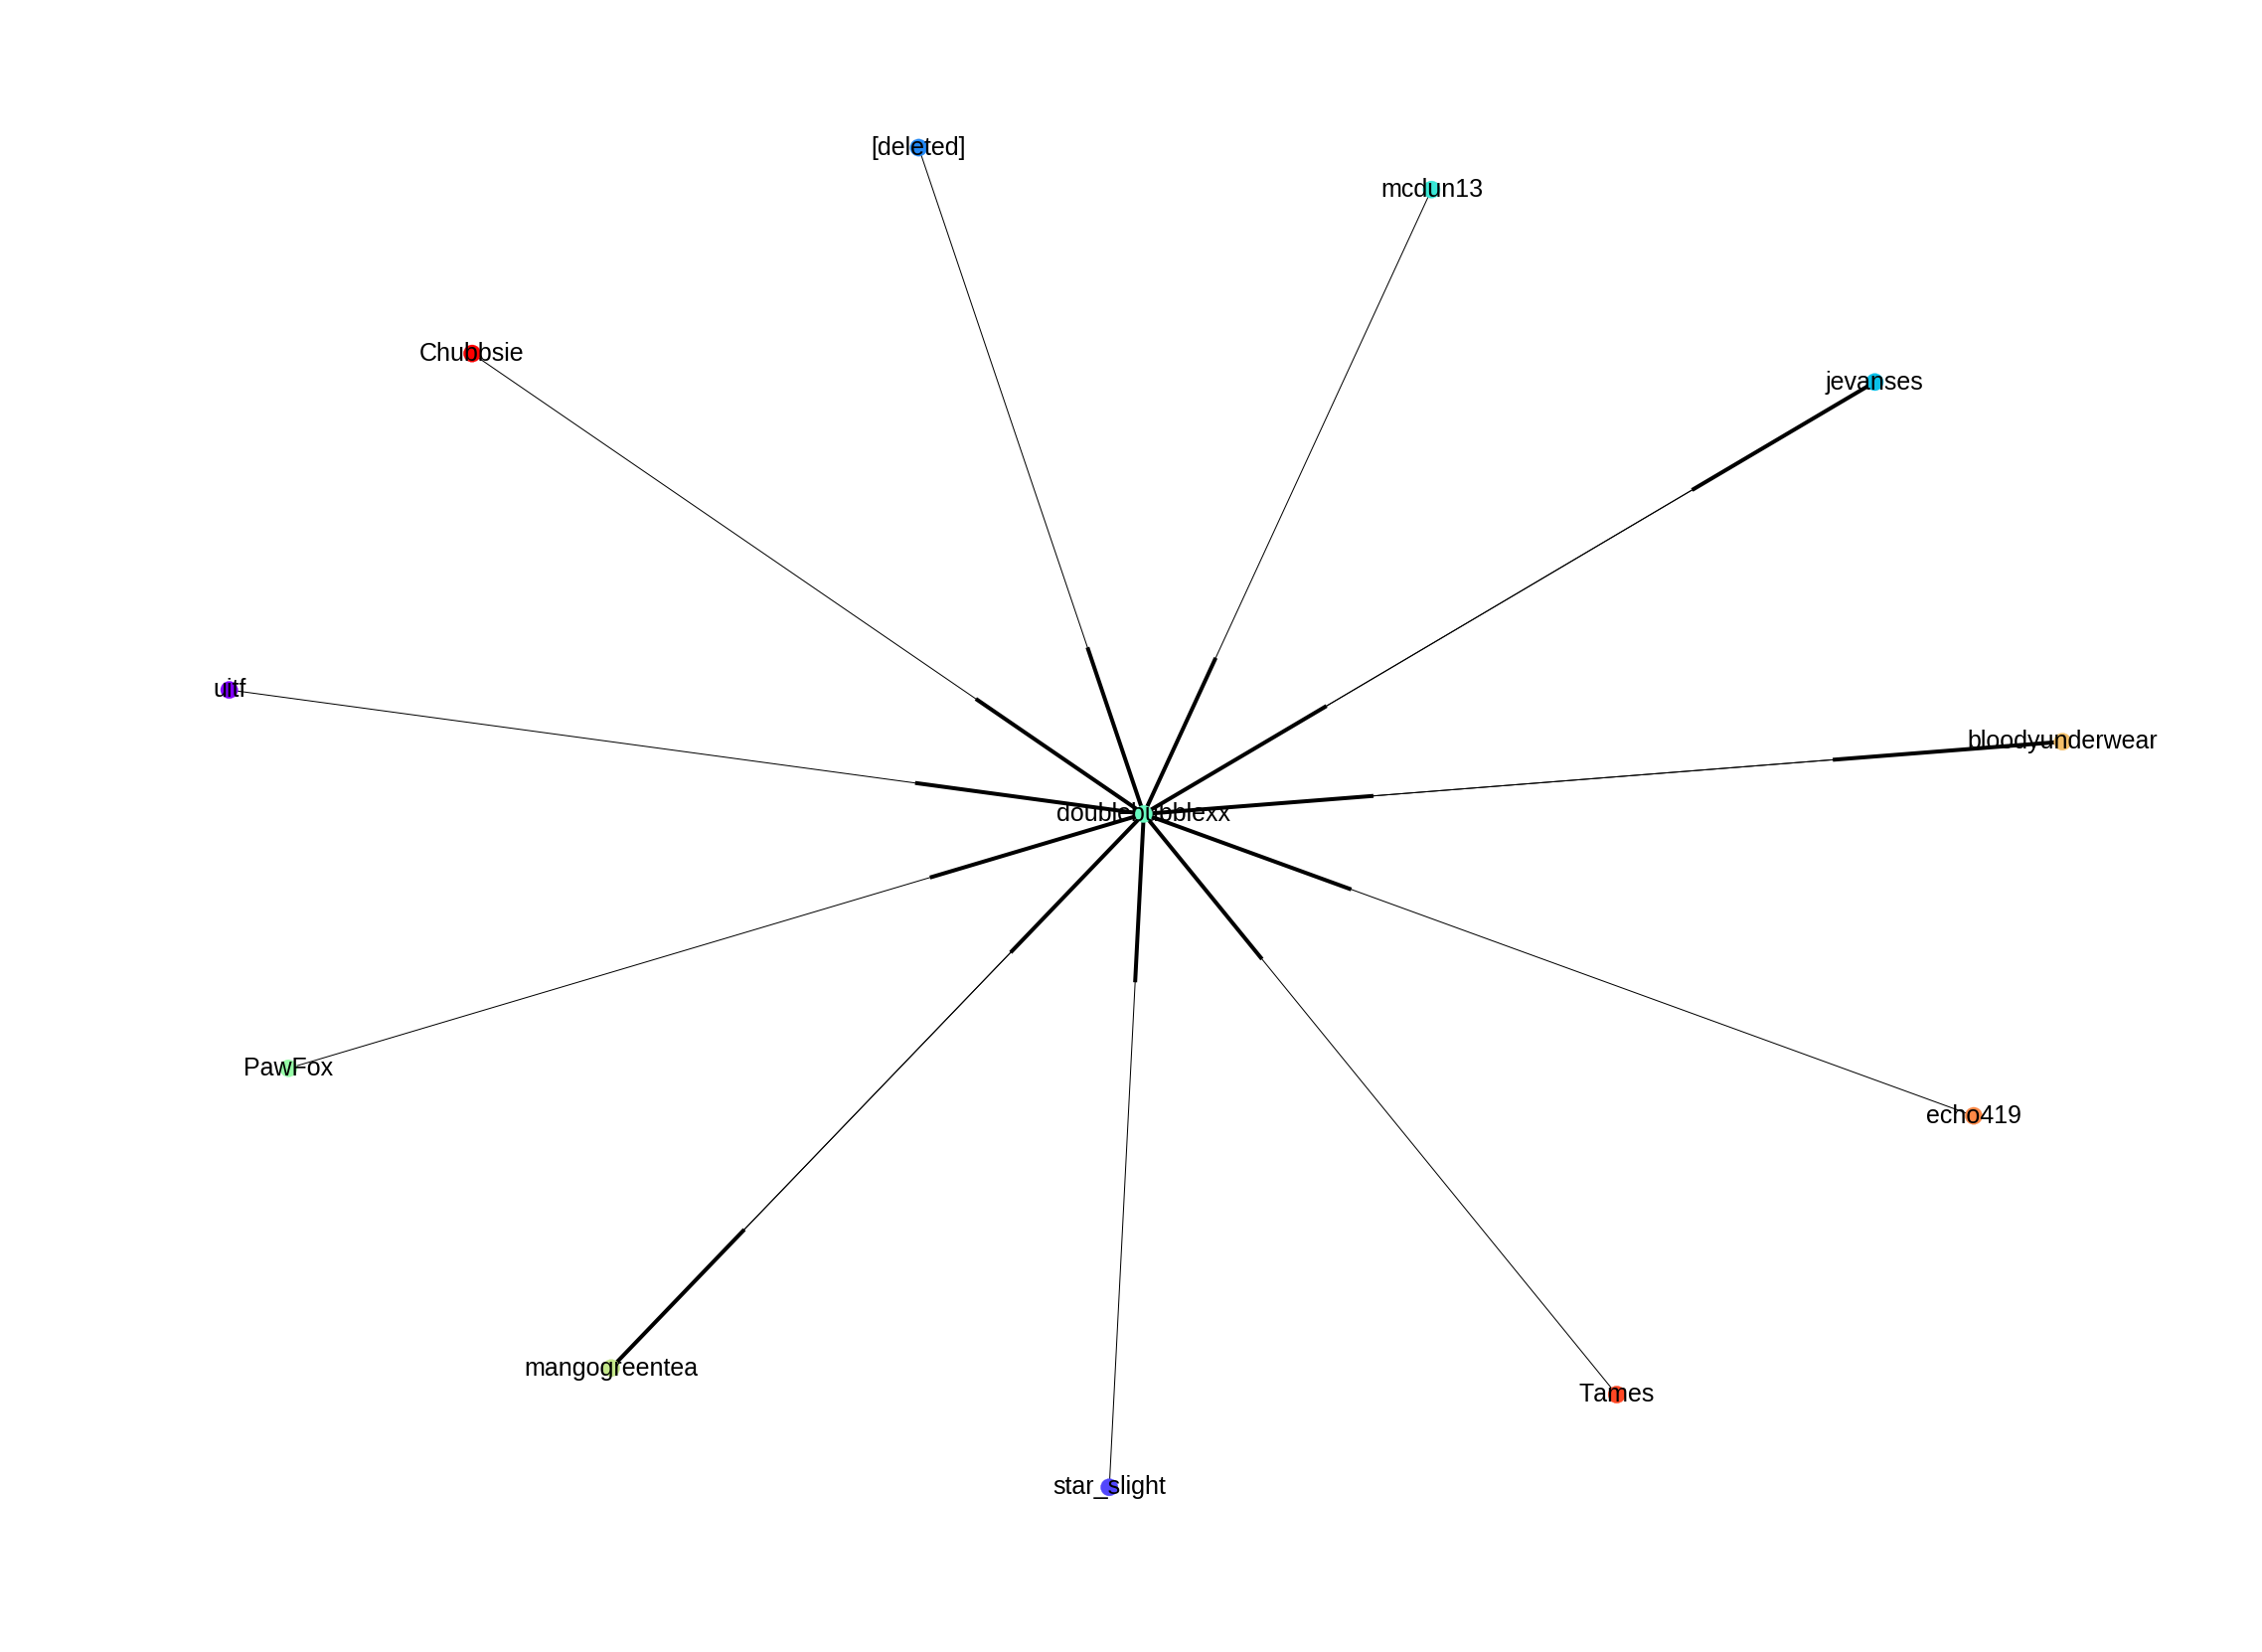
\includegraphics[width=0.45\linewidth, height = 5cm ]{Figures/UserGraphSW}
		\label{fig:uGraphSW}
	}


	\subfloat[]{
		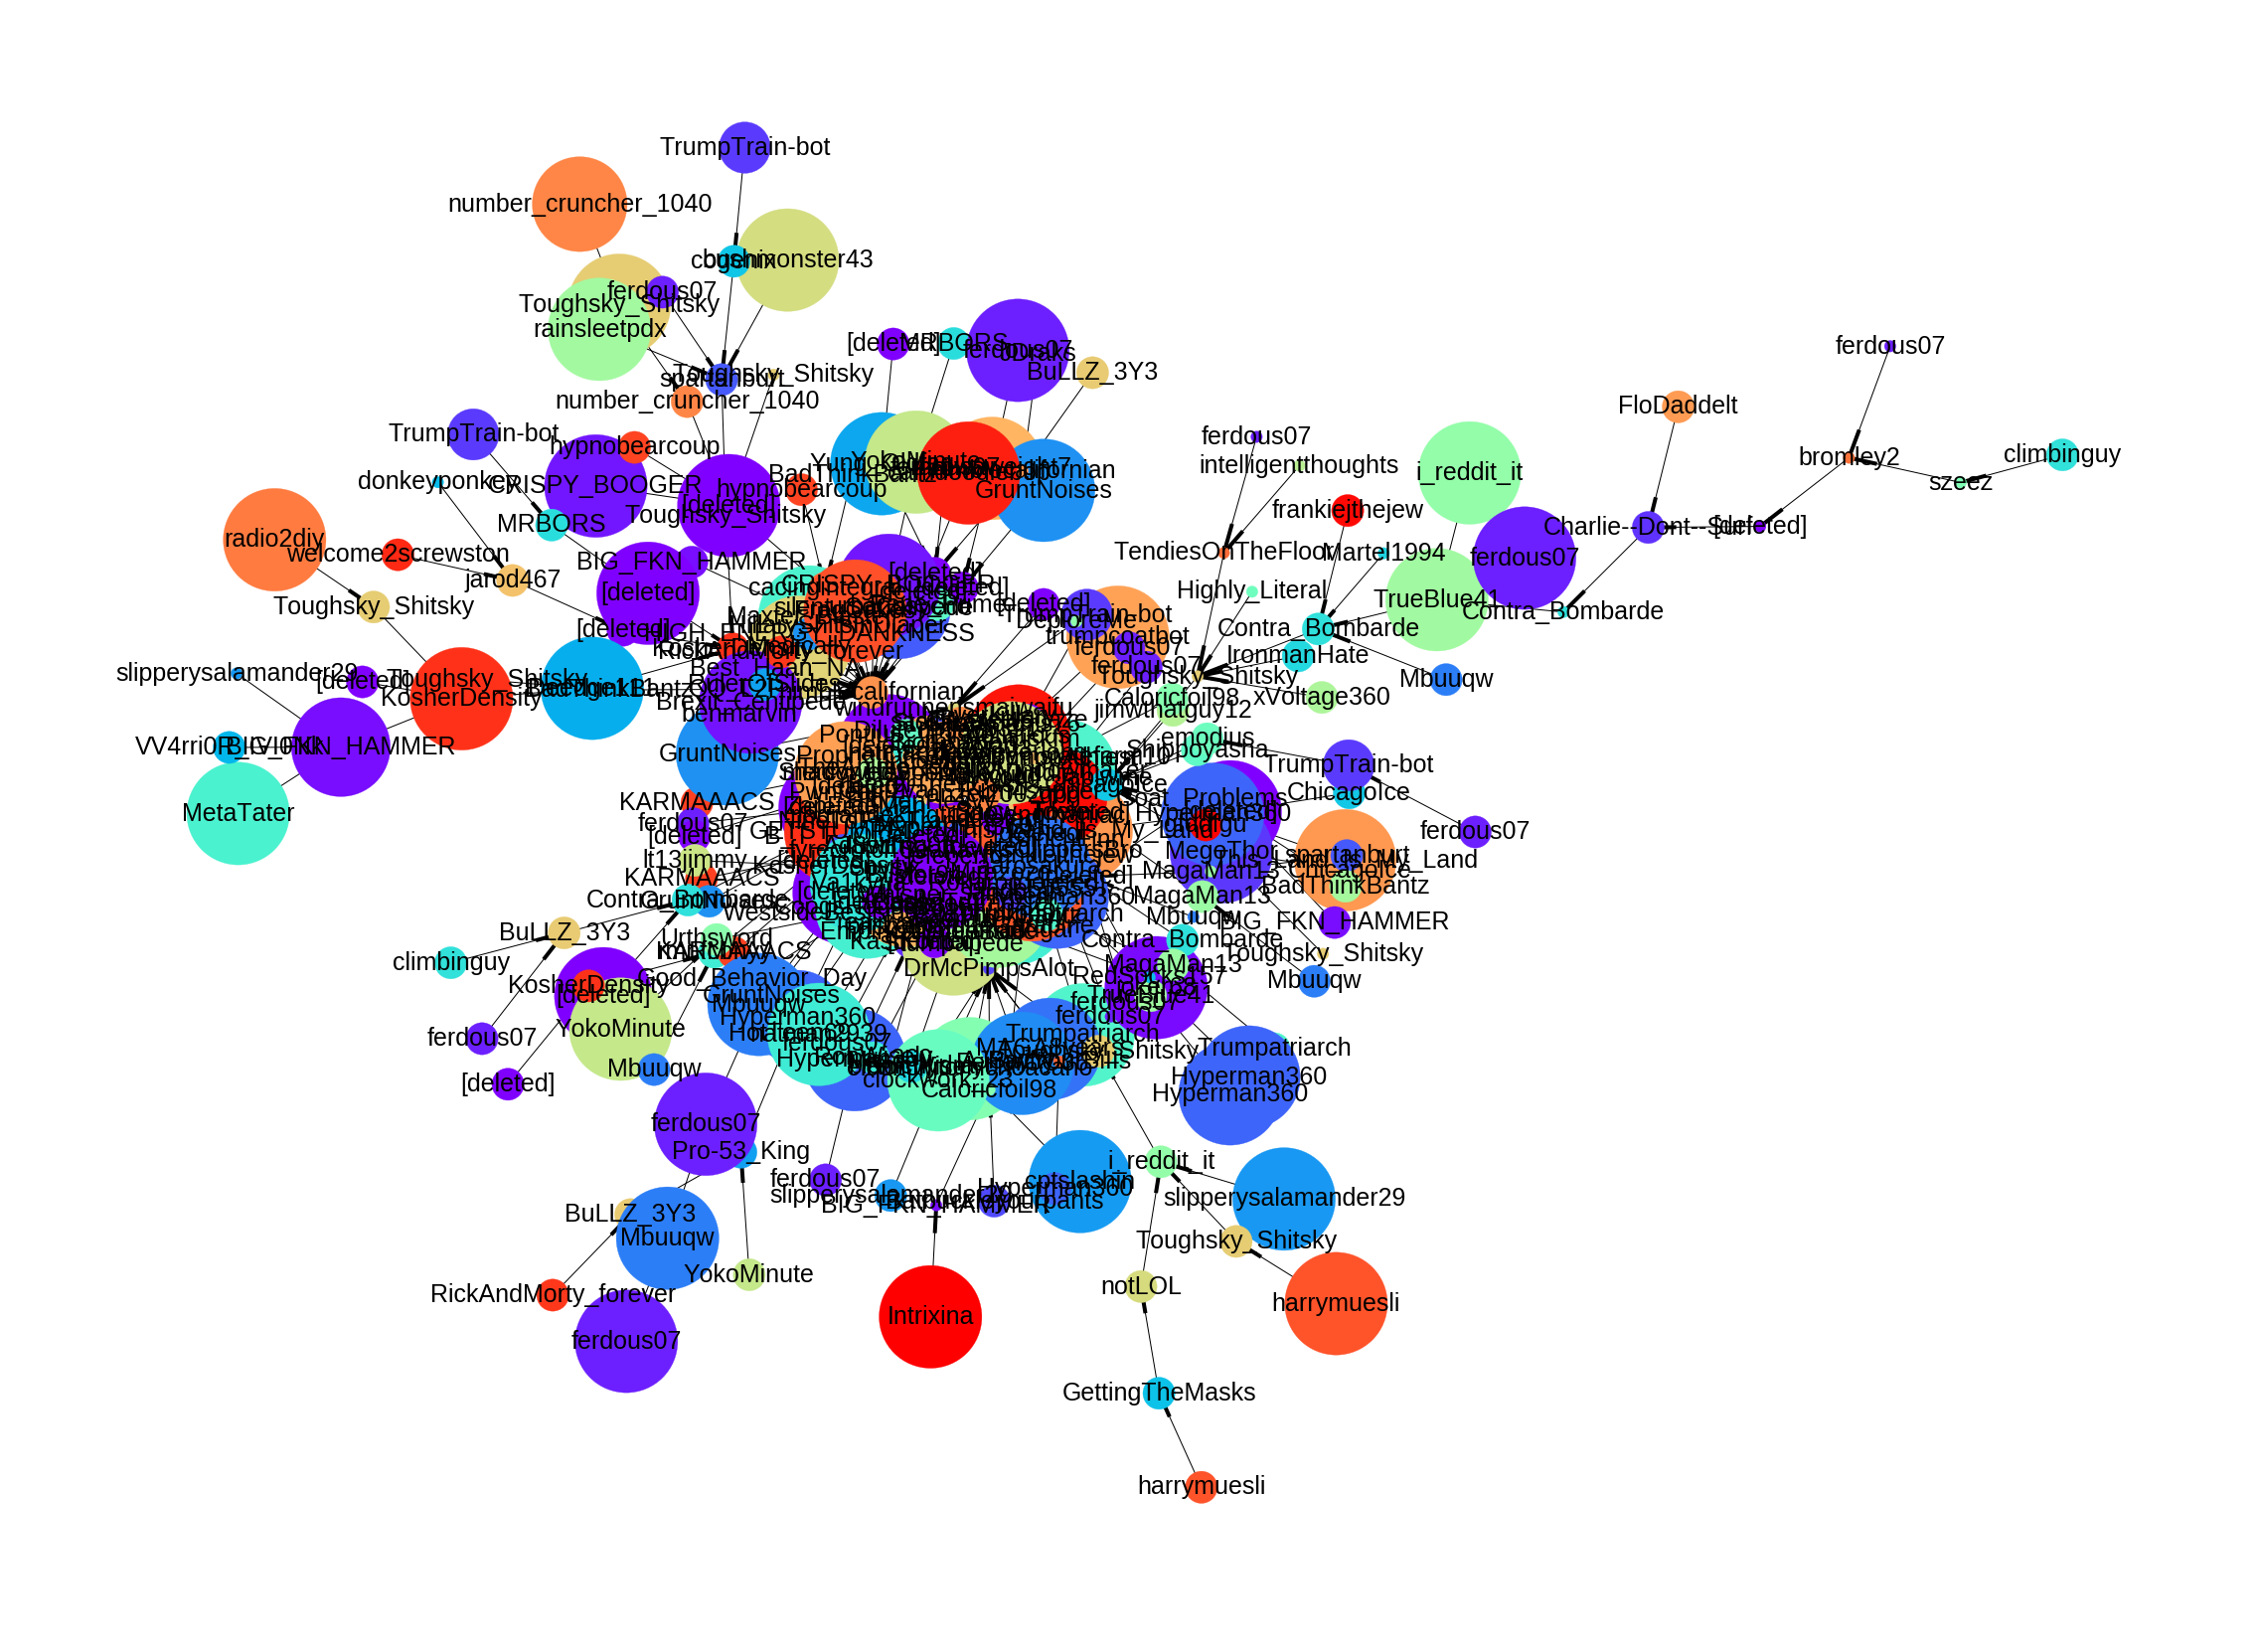
\includegraphics[width=0.45\linewidth, height = 5cm ]{Figures/ReplyGraphTD}
		\label{fig:rGraphTD}
	}
	\subfloat[]{
		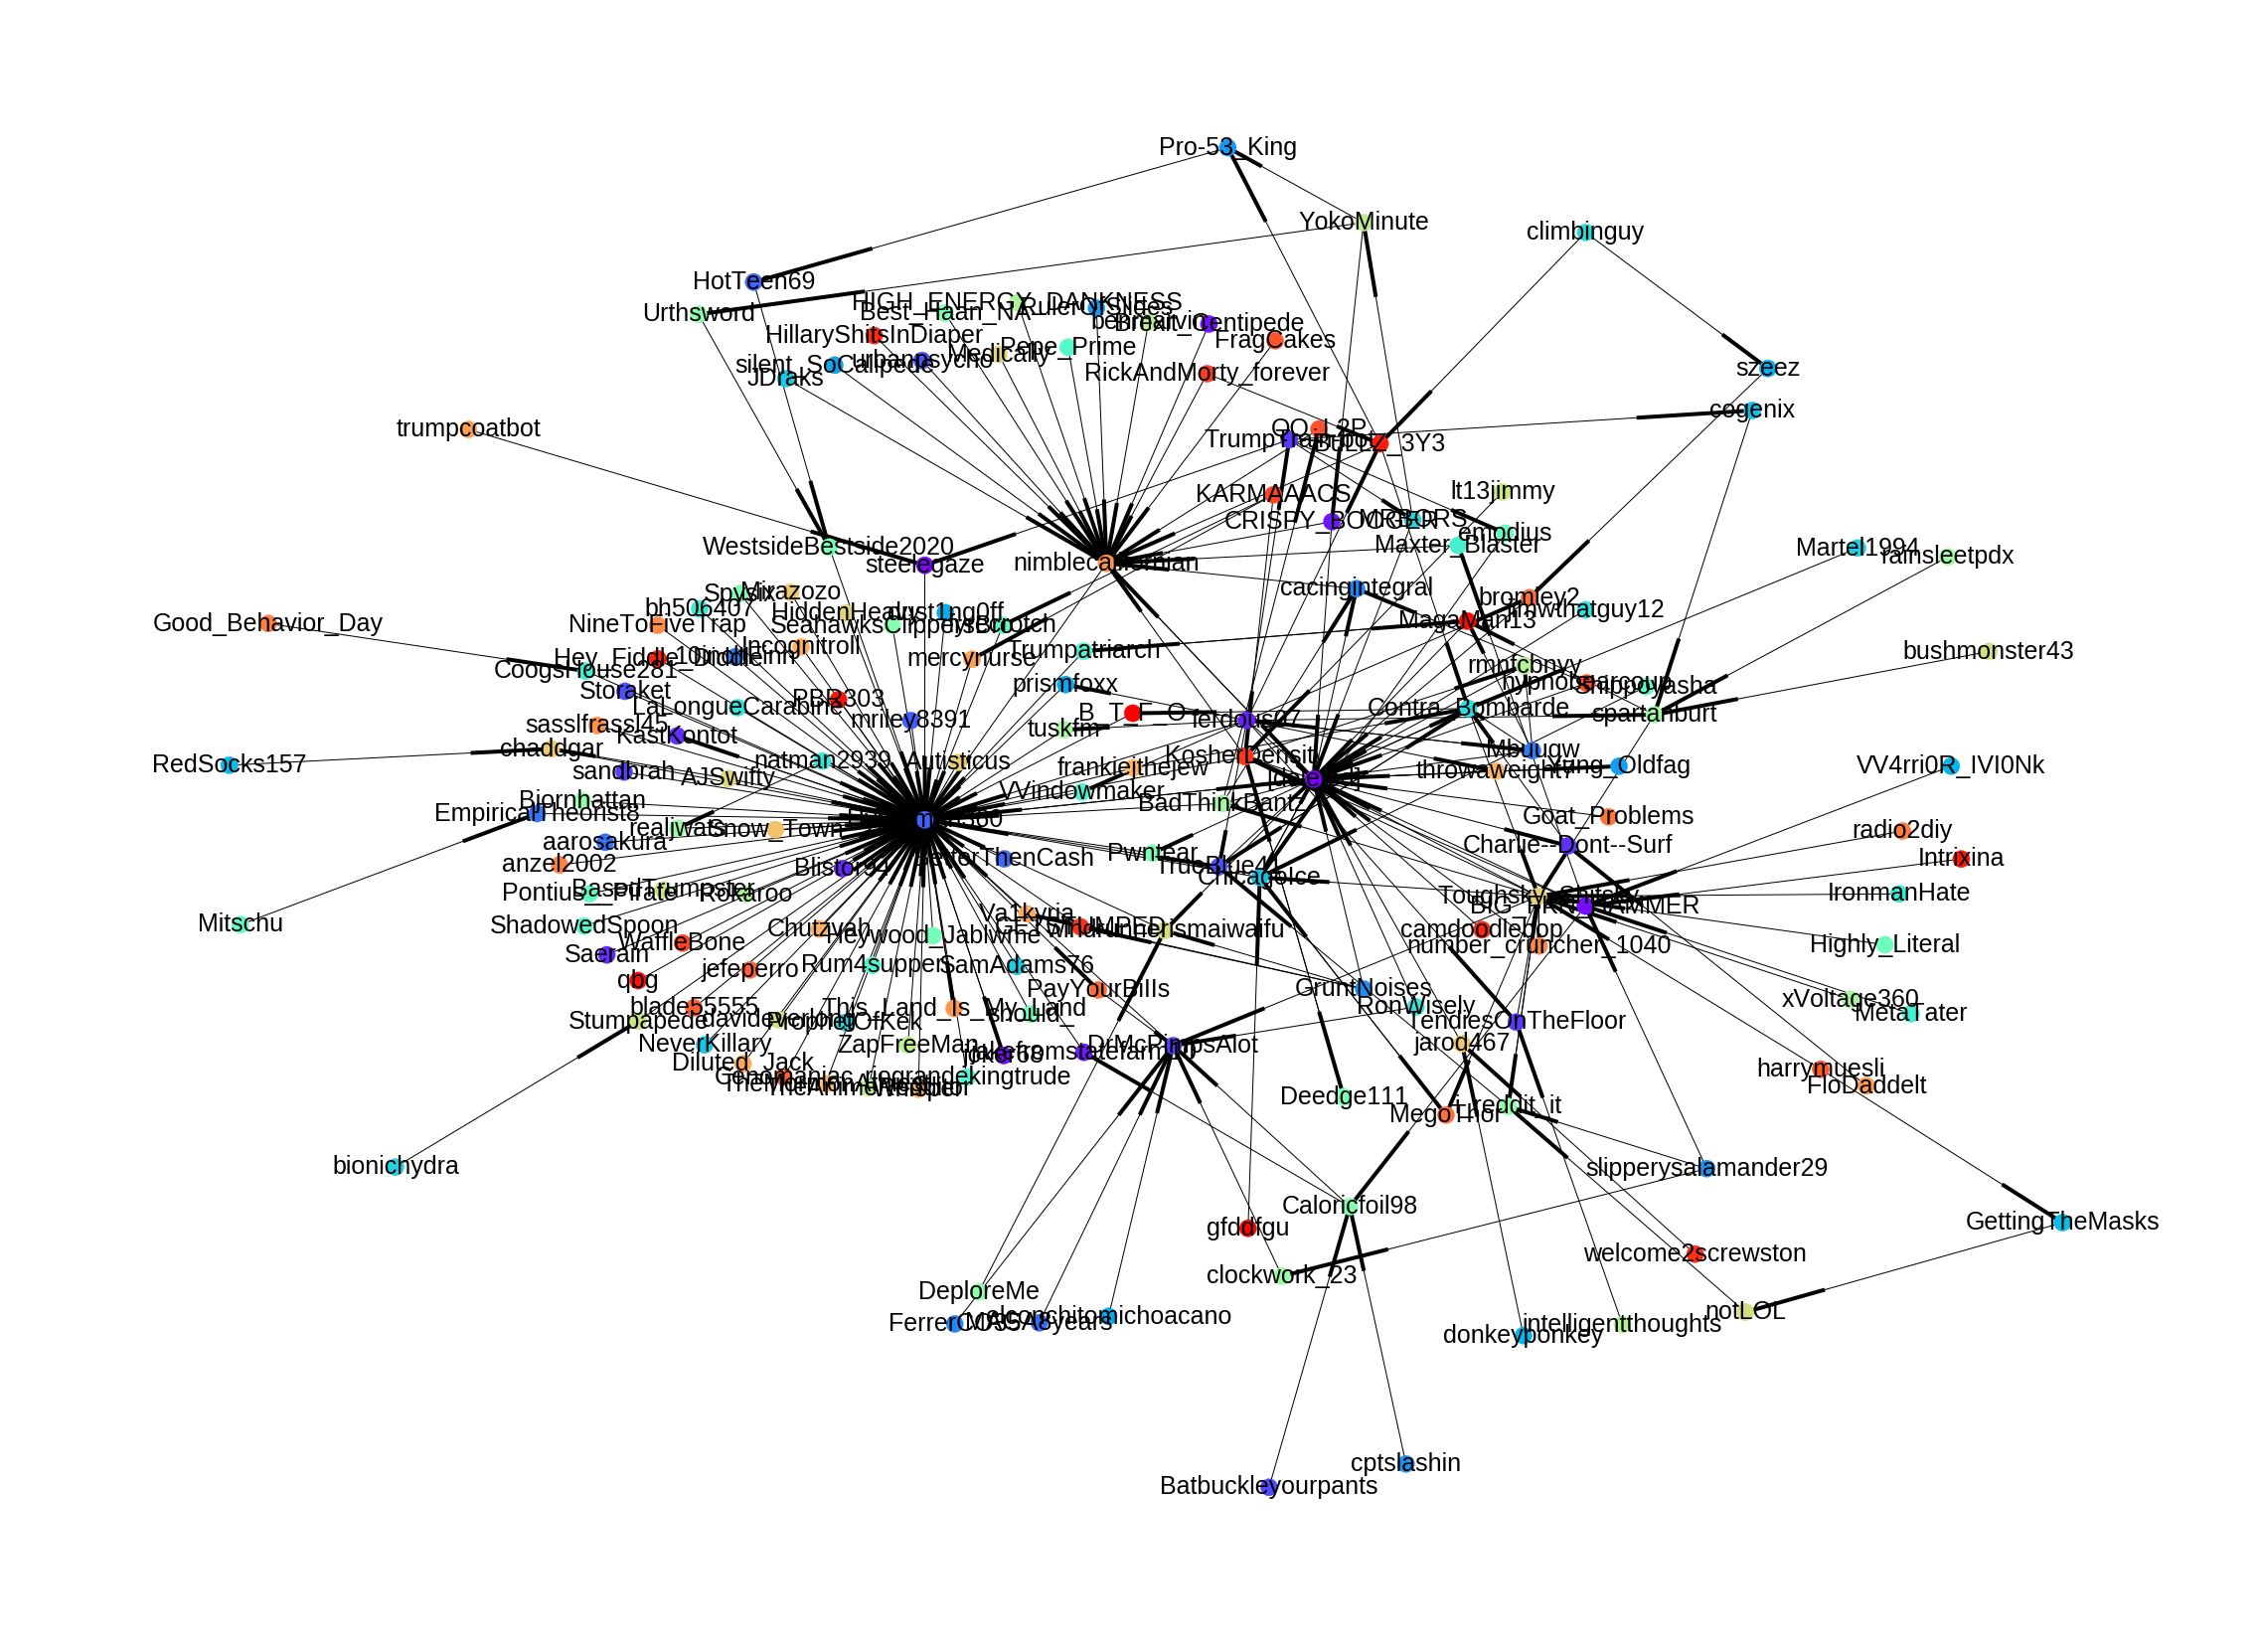
\includegraphics[width=0.45\linewidth, height = 5cm ]{Figures/UserGraphTD}
		\label{fig:uGraphTD}
	}
	\caption{ Example UserGraphs and their corresponding Reply graphs, Figure \ref{fig:uGraphSW} shows a random thread from the SW sub-reddit and \ref{fig:rGraphSW} shows the corresponding reply graph that arises from the response structure of the same thread. In comparison we have Usergraph Fig \ref{fig:uGraphTD} and its corresponding reply graph Fig \ref{fig:rGraphTD} from the subreddit r/TheDonald }
	\label{Fig:GraphExamples}
\end{figure*}

\subsection{Motif Extraction}
To understand relation of local structure in conversations with its nature, we compare the quantity called \textsl{motif occurrence ratio}. After calculating motif census across the dataset\cite{Batagelj2001}, we select progressive subsets of graphs from both datasets with nodes $n \in \{10 , 12 , 15 , 18 , 20 , 22 , 25 , 28 , 30\}$. For each of these node values we get a subset of graphs with those specific number of nodes, from Suicide watch and baseline frontpage, lets call then $\Gamma_{SW}$ and $\Gamma_{BL}$. Let us assume that for a given value of $n$ , $\Gamma_{SW}$ has $K_{SW}$ graphs and $\Gamma_{BL}$ has $K_{BL}$ graphs. We then count for a given motif, number of occurrences in $\Gamma_{SW}$ and $\Gamma_{BL}$ where the graph had at-least one instance of that motif. Let us call the total number of graphs in $\Gamma_{BL}$ with a given motif as $\gamma_{BL}$ and $\gamma_{SW}$ likewise for the $\Gamma_{SW}$ graphs. 
We then define the motif occurrence ratio as the fraction values for $\frac{\gamma_{BL}}{K_{BL}}$ and $\frac{\gamma_{SW}}{K_{SW}}$ for all the 16 motifs across all the chosen values of $n$. 


\bibliography{replyGraphs}
\end{document}
